\documentclass{beamer}
\usepackage{textpos}
\setlength{\TPHorizModule}{1cm} % Horizontale Einheit
\setlength{\TPVertModule}{1cm} % Vertikale Einheit
\usepackage{lmodern}
\usepackage{xcolor}
\usepackage{algpseudocode}
\usepackage{amsmath}
\usepackage{tcolorbox}
\usepackage{tikz}
\usepackage{tabularx, booktabs}
\usepackage{soul}
\usepackage{multirow}
\usepackage{gensymb}
\usepackage[normalem]{ulem} %for underline
\usepackage{adjustbox}
\usepackage{setspace}
\usepackage[font={scriptsize}, justification=centering, skip=0pt]{caption}
\usepackage[font={color=black},aboveskip=0pt]{subcaption}
\usepackage{ellipsis}
\usetikzlibrary{decorations.pathmorphing,calc}
\usetikzlibrary{decorations.pathreplacing}
\usetikzlibrary{positioning}
\usepackage{chemarrow}
\usepackage{slashbox}
\usepackage[ruled,vlined,linesnumbered]{algorithm2e}
\usepackage{siunitx}
\usepackage{relsize}
\usepackage{3dplot}
\usepackage{threeparttable}
\usetikzlibrary{fit}
\usepackage[utf8]{inputenc}
\usepackage[upright]{fourier}
\usetikzlibrary{matrix,arrows,decorations.pathmorphing}
\usepackage{xparse}
\beamertemplatenavigationsymbolsempty
\usepackage[nomessages]{fp}% http://ctan.org/pkg/fp
\usetikzlibrary{calc}
\usepackage{breqn} %for dmath
\usepackage{hyperref} 
\usepackage{arydshln}
% for: large cdots:http://tex.stackexchange.com/questions/235118/making-a-thicker-cdot-for-dot-product-that-is-thinner-than-bullet 
\makeatletter
\newcommand*\bigcdot{\mathpalette\bigcdot@{.5}}
\newcommand*\bigcdot@[2]{\mathbin{\vcenter{\hbox{\scalebox{#2}{$\m@th#1\bullet$}}}}}
\makeatother
% endfor
\newcommand\reduline{\bgroup\markoverwith
    {\textcolor{red}{\rule[-0.5ex]{2pt}{0.8pt}}}\ULon
}
\usetikzlibrary{shapes,fit}
\definecolor{univred}{rgb}{0.7, 0.0, 0.0}
\definecolor{drkgreen}{rgb}{0,0.26,0.15}
\definecolor{aureolin}{rgb}{0.99,0.93,0.0}
\DeclareMathOperator*{\argmax}{argmax}
%
%
\newcolumntype{C}[1]{>{\centering\let\newline\\\arraybackslash\hspace{0pt}}m{#1}}
\setbeamertemplate{background canvas}{%
    {\color{univred}\noindent\makebox[\paperwidth]{\rule{\paperwidth}{2.5ex}}}
}
\setbeamertemplate{frametitle}{\color{black}\bfseries\vskip2ex\insertframetitle\par\vskip-6pt\hrulefill}
\addtobeamertemplate{frametitle}{}{%
%CMU logo in header
    \begin{textblock*}{100mm}(0.87\textwidth,-1.425cm)
        \includegraphics[height=1.5cm,width=1.9cm,keepaspectratio]{cm_logo}
    \end{textblock*}
%ECE logo in footer
    \begin{textblock*}{10mm}(-.8cm,7.5cm)
        \includegraphics[height=2cm,width=2.5cm,keepaspectratio]{ece}
    \end{textblock*}
}
%\addtobeamertemplate{footnote}{}{\vspace{2ex}}
\setbeamercolor*{item}{fg=black}
% The line below doesn't hide the total frame number, so using 
% http://tex.stackexchange.com/a/32815/32460 
%\setbeamertemplate{footline}[page number]{}
\makeatletter
\setbeamertemplate{footline}
{
    \leavevmode%
    \hbox{%
%\setbeamercolor{page number in head/foot}{fg=univred}
        \begin{beamercolorbox}[wd=.98\paperwidth,ht=2.25ex,dp=1ex,right]{date in head/foot}%
            \insertframenumber\hspace*{2ex} 
        \end{beamercolorbox}
    }%
    \vskip0pt%
}
\makeatother

\newlength\MyColSep
\setlength\MyColSep{1cm}
\newlength\MyColWd
\setlength\MyColWd{0.3333\textwidth-0.6666666\MyColSep}

\let\otp\titlepage
\renewcommand{\titlepage}{\otp\addtocounter{framenumber}{-1}}

\title{\color{univred} A Comparison of Antenna Placement Algorithms}
\author{Abhinav Jauhri}
\date{\today}
\begin{document}
\begin{frame}[plain]
%CMU logo in header
    \begin{textblock*}{100mm}(0.87\textwidth,-1.15cm)
        \includegraphics[height=1.5cm,width=1.9cm,keepaspectratio]{cm_logo}
    \end{textblock*}
    \begin{textblock*}{10mm}(-.8cm,7.78cm)
        \includegraphics[height=2cm,width=2.5cm,keepaspectratio]{ece}
    \end{textblock*}
    \color{univred}
    \titlepage
\end{frame}

\begin{frame}{Motivation}
\begin{itemize} \itemsep1.5em
        \item Antenna placement study is often ignored 
        \item Placing new antennas requires a long, manual effort to complete an antenna placement study, if at all
        \item Parasitic effects due to fixed or mobile platform 
        \item With multiple antennas systems offer interference, and thereby reduce each antenna's efficiency
    \end{itemize}
    \vspace{5mm}
\end{frame}

\begin{frame}{Outline of this talk}
    \begin{itemize}
        \setlength\itemsep{2em}
        \item Part 1: Introduction to the antenna placement problem
        \item Part 2: Description of stochastic algorithms, their properties and operators
        \item Part 3: Evaluation of test cases
    \end{itemize}
\end{frame}

\begin{frame}{\null}
    \begin{tcolorbox}[colback=green!5]
        \centering\Huge
        Part 1: Introduction to the antenna placement problem
    \end{tcolorbox}
\end{frame}

\begin{frame}{Antenna Placement Problem}
    \centering
    \begin{columns}
        \column{0.33\linewidth}
        \only<1->{
            \begin{textblock}{3}(0.2,-2.8) Given, platform \end{textblock}
            \begin{textblock}{3}(0.2,-1.9)
                \begin{figure}
                    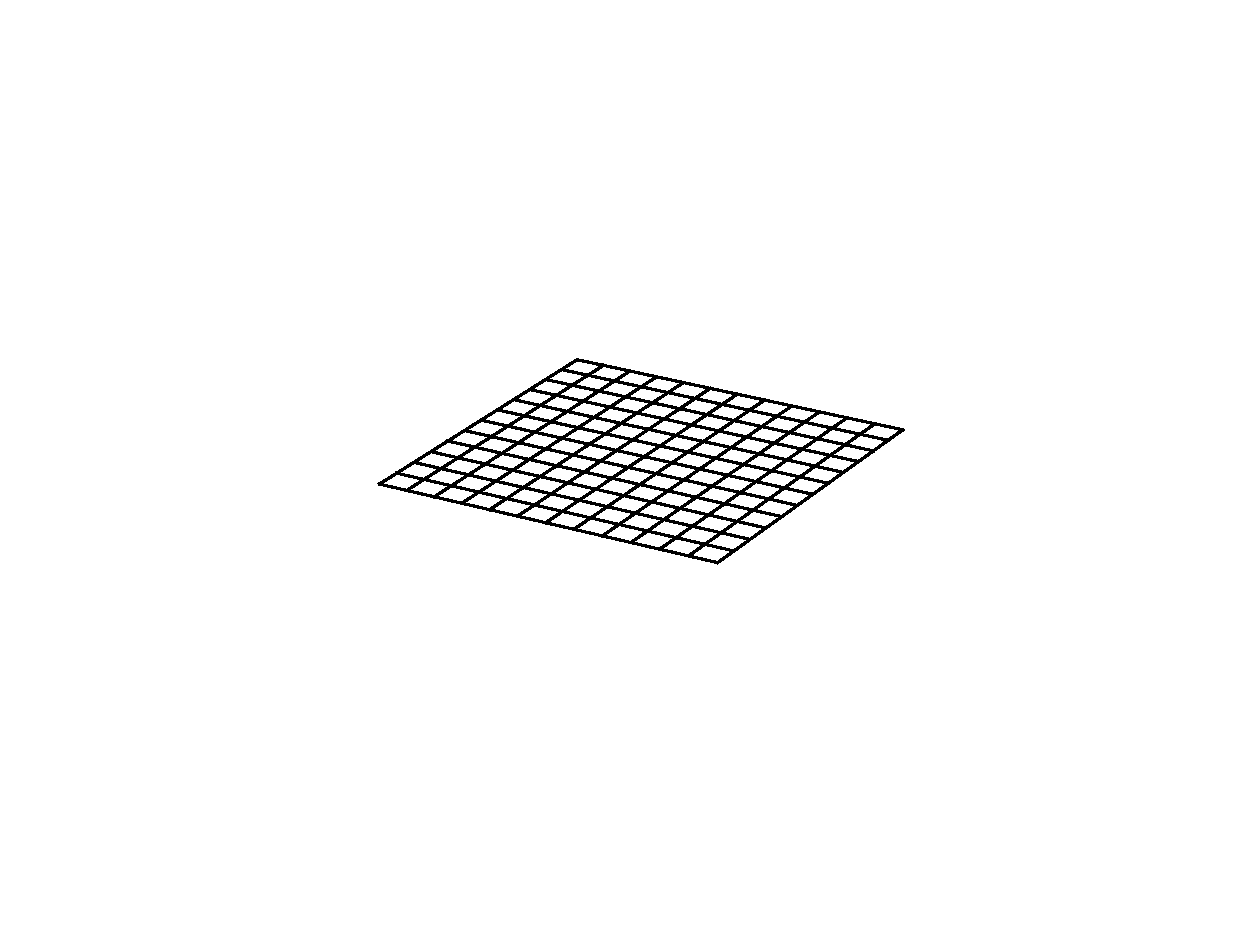
\includegraphics[trim=175 165 140 165, clip, scale=0.4]{../paper/FIG/tc1_platform}
                \end{figure}\end{textblock}
        }
        \only<2->{
            \begin{textblock}{9}(-1,1)\textbf{Problem:} Find best antenna placements to maximize gain and minimize coupling \end{textblock}
            \begin{textblock}{3}(2.5,1.5)
                \begin{figure}
                    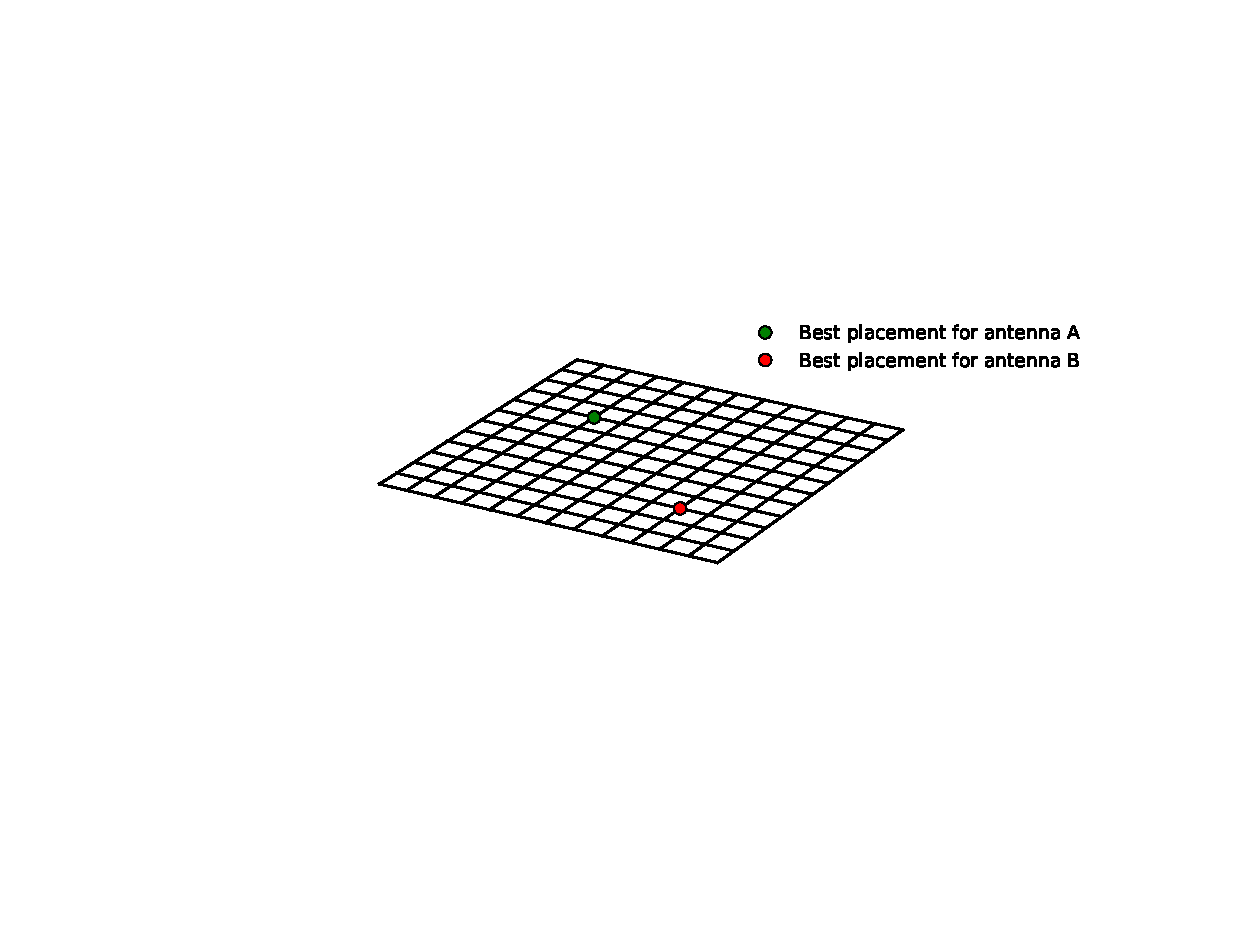
\includegraphics[trim=170 165 65 145, clip, scale=0.4]{../paper/FIG/tc11_intro}
                \end{figure}\end{textblock}
        }
        \column{0.33\linewidth}
        \only<1->{
            \begin{textblock}{6}(-1.5,-2.8) + \end{textblock}
            \begin{textblock}{6}(-0.7,-2.8) allowable placements of antennas \end{textblock}
            \begin{textblock}{3}(-0.2,-2)
                \begin{figure}
                    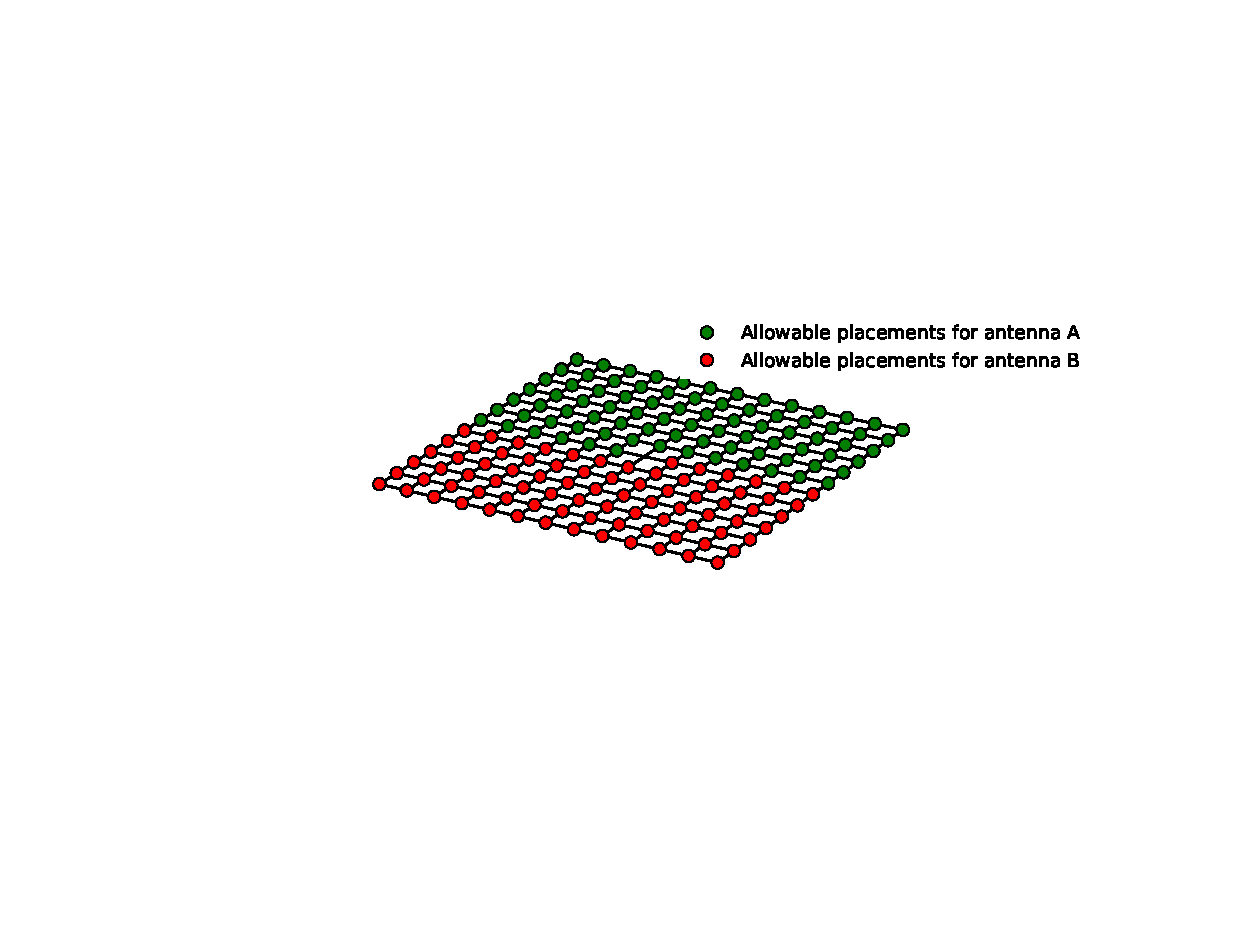
\includegraphics[trim=170 165 65 145, clip, scale=0.4]{../paper/FIG/tc1_intro}
                \end{figure}\end{textblock}
        }
    \end{columns}
\end{frame}

\begin{frame}[t]{Antenna Placement Problem}
    Given:
\begin{itemize} \itemsep1.5em
        \item platform $P$ with its surface gridded such that end points represent possible antenna placements
        \item set of  $n$ antennas $A = {A_1, A_2, \dots, A_n}$ such that $n > 1$
        \item for each $A_i$, $L_i$ denote the set of allowable placements $\in \mathbb R^3$ such that $\mid L_i \mid = m_i$ and $\forall i, m_i > 1$\[ L_i = \{(x_{1}, y_{1}, z_{1}) \dots (x_{m_i}, y_{m_i}, z_{m_i})\} \]
    \end{itemize}
    \textbf{Problem}: Find a set of $n$ optimal antenna placements on $P$ to maximize gain and minimize coupling. \\
    \vspace*{2mm}
    \textbf{Size of search space} $= \mathbf{m^n}$, if $m_i = m, \forall i \in [1,n]$
\end{frame}

\begin{frame}{\null}
    \begin{tcolorbox}[colback=green!5]
        \centering
        Question: How is a good antenna placement quantified in the context of platform and other antennas?
    \end{tcolorbox}
\end{frame}

\begin{frame}[t]{Mutual Coupling}
    When two antennas are in proximity, and one is transmitting, the second will receive some of the transmitted power.\\ \vspace{2mm}
    \begin{figure}\centering
        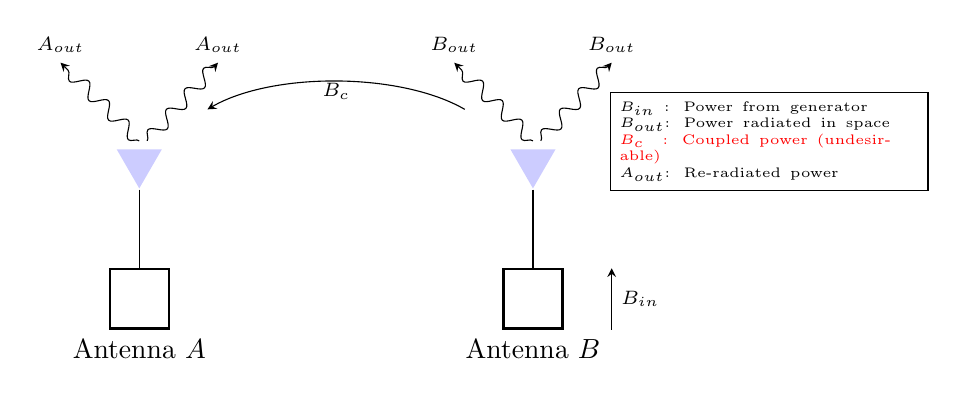
\begin{tikzpicture} [
                triangle/.style = {fill=blue!20, regular polygon, regular polygon sides=3 },
                node rotated/.style = {rotate=180},
                border rotated/.style = {shape border rotate=180}
            ]
            \node (b1) at (0, 1) [draw,thick,minimum width=.75cm,minimum height=.75cm, label=below:Antenna $A$] {}; 
            \node[triangle, border rotated, above=1cm of b1] (a1) {};
            \draw [-] (a1) -- (b1);
            \node (b2) at (5, 1) [draw,thick,minimum width=.75cm,minimum height=.75cm, label=below:Antenna $B$] {}; 
            \node[triangle, border rotated, above=1cm of b2] (a2) {};
            \draw [-] (a2) -- (b2);
            \draw [-stealth] ([xshift=1cm] b2.south) to node[right] {\scriptsize $B_{in}$} ([xshift=1cm] b2.north);
            \draw [stealth-, shorten <= 1cm, shorten >= 1cm] (a1.north) to[bend left] node {\scriptsize $B_c$} (a2.north);
            \draw [-stealth,decorate,decoration=snake] ([yshift=.1cm, xshift=.1cm] a1.north) -- (1,4) node[above] {\scriptsize $A_{out}$};
            \draw [-stealth,decorate,decoration=snake] ([yshift=.1cm] a1.north) -- (-1,4) node[above] {\scriptsize $A_{out}$};
            \draw [-stealth,decorate,decoration=snake] ([yshift=.1cm, xshift=.1cm] a2.north) -- (6,4) node[above] {\scriptsize $B_{out}$};
            \draw [-stealth,decorate,decoration=snake] ([yshift=.1cm] a2.north) -- (4,4) node[above] {\scriptsize $B_{out}$};
            \node[draw, text width=3.8cm] at (8,3) {\tiny $B_{in}~$:  Power from generator\\$B_{out}$: Power radiated in space\\{\color{red}$B_c~~$: Coupled power (undesirable)}\\$A_{out}$: Re-radiated power\\}; 
        \end{tikzpicture}
    \end{figure}
\end{frame}

\begin{frame}{Minimize Mutual Coupling (MC)}
    \begin{tcolorbox}[colback=green!5]
        \begin{equation}
            F_{MC} = \sum_{i=1}^{n-1}\sum_{j=i+1}^{n} CP(A_i, A_j),
        \end{equation}
    \end{tcolorbox}
    where
    \begin{itemize}
        \item $CP(\cdot, \cdot) \in \mathbb R$ is the coupling between two antennas, and computed using a simulator
        \item There will be $n \choose 2$ coupling terms 
    \end{itemize}
    \vspace{2mm}
    \small\textit{Example:} If $n=3$, then $F_{MC} = CP(A_1, A_2) + CP(A_1, A_3) + CP(A_2, A_3)$
\end{frame}

\begin{frame}{Free Space Gain Pattern / Radiation Pattern}
    \begin{columns}
        \begin{column}{0.5\linewidth}
            \begin{figure}
                \vspace{-2.5cm}
                \centering
                \includegraphics[width=4cm, height=5cm]{../paper/FIG/free_space.png}
                \caption*{\tiny Free-space pattern without platform or other antennas}
            \end{figure}
        \end{column}
        \begin{column}{0.5\linewidth}
            \begin{overlayarea}{\textwidth}{\textheight}
                \begin{figure}
                    \begin{subfigure}{\columnwidth}
                        \centering
                        \includegraphics[scale=0.3]{../paper/FIG/free_cross.png}
                        \caption*{\tiny 2D view of the \textcolor{blue}{free-space gain pattern}}%
                    \end{subfigure}\vspace*{2mm}
                    \begin{tcolorbox}[colback=green!5]
                        \centering
                        This is ideal pattern since there is no interference
                    \end{tcolorbox}
                \end{figure}
            \end{overlayarea}
        \end{column}
    \end{columns}
\end{frame}

\begin{frame}{Gain Pattern}
    \begin{columns}
        \begin{column}{0.5\linewidth}
            \begin{figure}
                \vspace{-2.5cm}
                \centering
                \includegraphics[width=4cm, height=5cm]{../paper/FIG/free_space.png}
                \caption*{\tiny Free-space pattern without platform or other antennas}
            \end{figure}
        \end{column}
        \begin{column}{0.5\linewidth}
            \begin{overlayarea}{\textwidth}{\textheight}
                \begin{figure}
                    \begin{subfigure}{\columnwidth}
                        \centering
                        \includegraphics[scale=0.3]{../paper/FIG/free_cross.png}
                        \caption*{\tiny {2D view of the \textcolor{blue}{free-space gain pattern}}}%
                    \end{subfigure}\vspace*{2mm}
                    \begin{subfigure}{\columnwidth}
                        \centering
                        \includegraphics[scale=0.3]{../paper/FIG/comp_cross.png}
                        \caption*{\tiny {\textcolor{red}{In-situ gain pattern} for random antenna placement different from \textcolor{blue}{free-space gain pattern}}}%
                    \end{subfigure}
                \end{figure}
            \end{overlayarea}
        \end{column}
    \end{columns}
\end{frame}



\begin{frame}{Minimize Difference in Gain Pattern (GP)}
    \begin{tcolorbox}[colback=green!5]
        \begin{equation} \label{eq:rp}
            F_{GP} = \sum_{i=1}^n~\sum_{\theta=0}^{\frac{180\degree}{S}}~\sum_{\phi=0}^{\frac{360\degree}{S}}
            \left( FSG_i(S\theta,S\phi) - ISG_i(S\theta,S\phi) \right) ^2,
        \end{equation}
    \end{tcolorbox}
    where
    \begin{itemize}
            \small
        \item $S$ is the step size
        \item $\theta, \phi$ spherical coordinates in degrees
        \item $FSG(\cdot,\cdot) \in \mathbb R$ is the free-space gain pattern computed by the simulator
        \item $ISG(\cdot,\cdot) \in \mathbb R$ is the in-situ gain pattern computed by the simulator
    \end{itemize}
\end{frame}

\begin{frame}{Fitness Evaluation}
    Find a placement configuration such that \textbf{fitness $F$} is minimal:
    \vspace*{.5cm}
    \begin{tcolorbox}[colback=green!5]
        \begin{equation} \label{eq:optimal}
            F = \alpha F_{MC} + \beta F_{GP},
        \end{equation}
    \end{tcolorbox}
    where $\alpha,~ \beta$ are adjustable weights for each of the objectives 
\end{frame}

\begin{frame}{\null}
    \begin{tcolorbox}[colback=green!5]
        \centering\Huge
        Part 2: Stochastic Algorithms
    \end{tcolorbox}
\end{frame}

\begin{frame}[t]{Individual(s)}
    An \textbf{individual} is a member of a set of feasible solutions.
\begin{itemize} \itemsep1.5em
        \item Algorithm operates on an individual:\\
            \adjustbox{valign=t}{%
                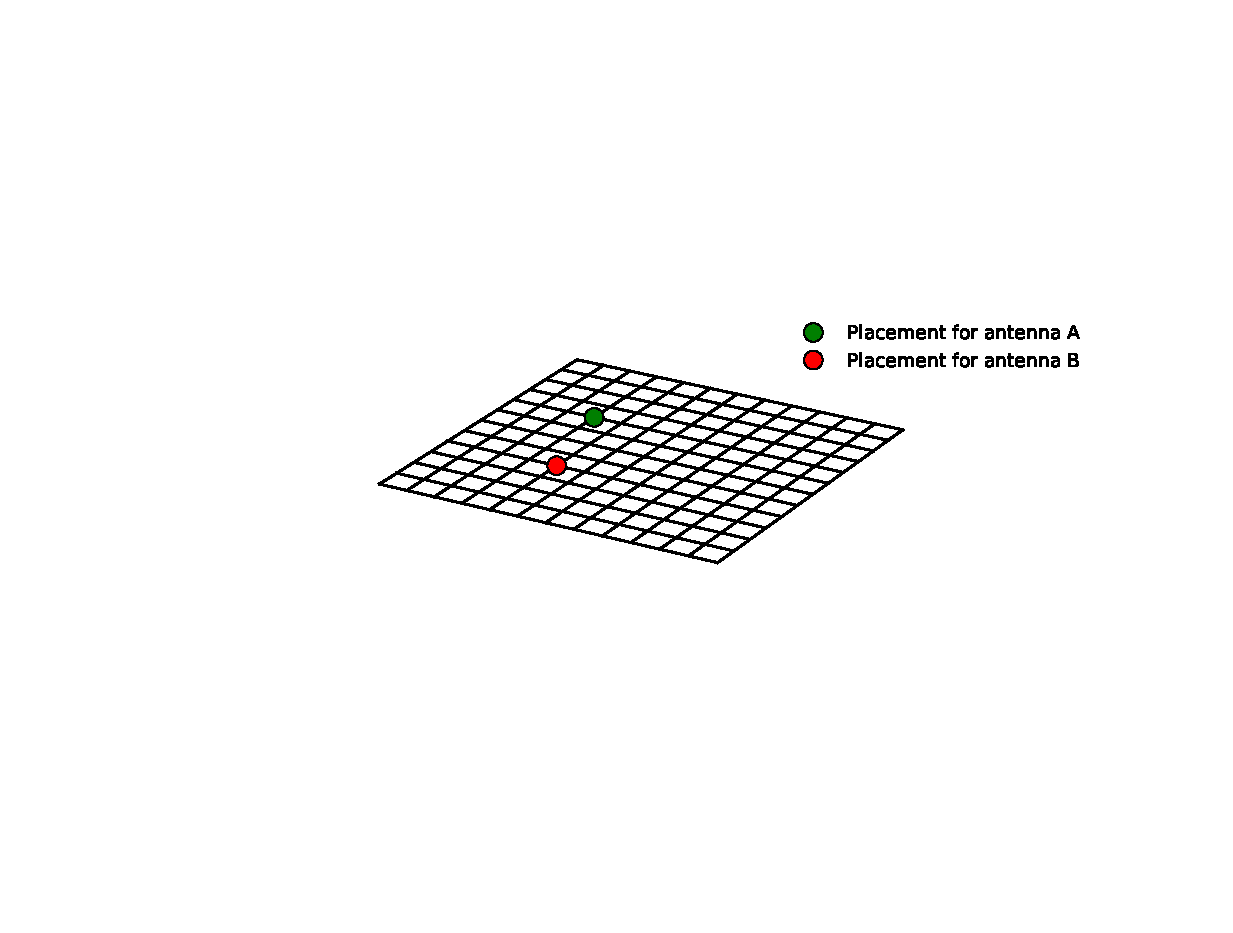
\includegraphics[trim=125 165 50 135, clip, scale=0.35]{../paper/FIG/tc1_mut3}
            }
        \item Some algorithms operate on a population of individuals:
            \adjustbox{valign=t}{%
                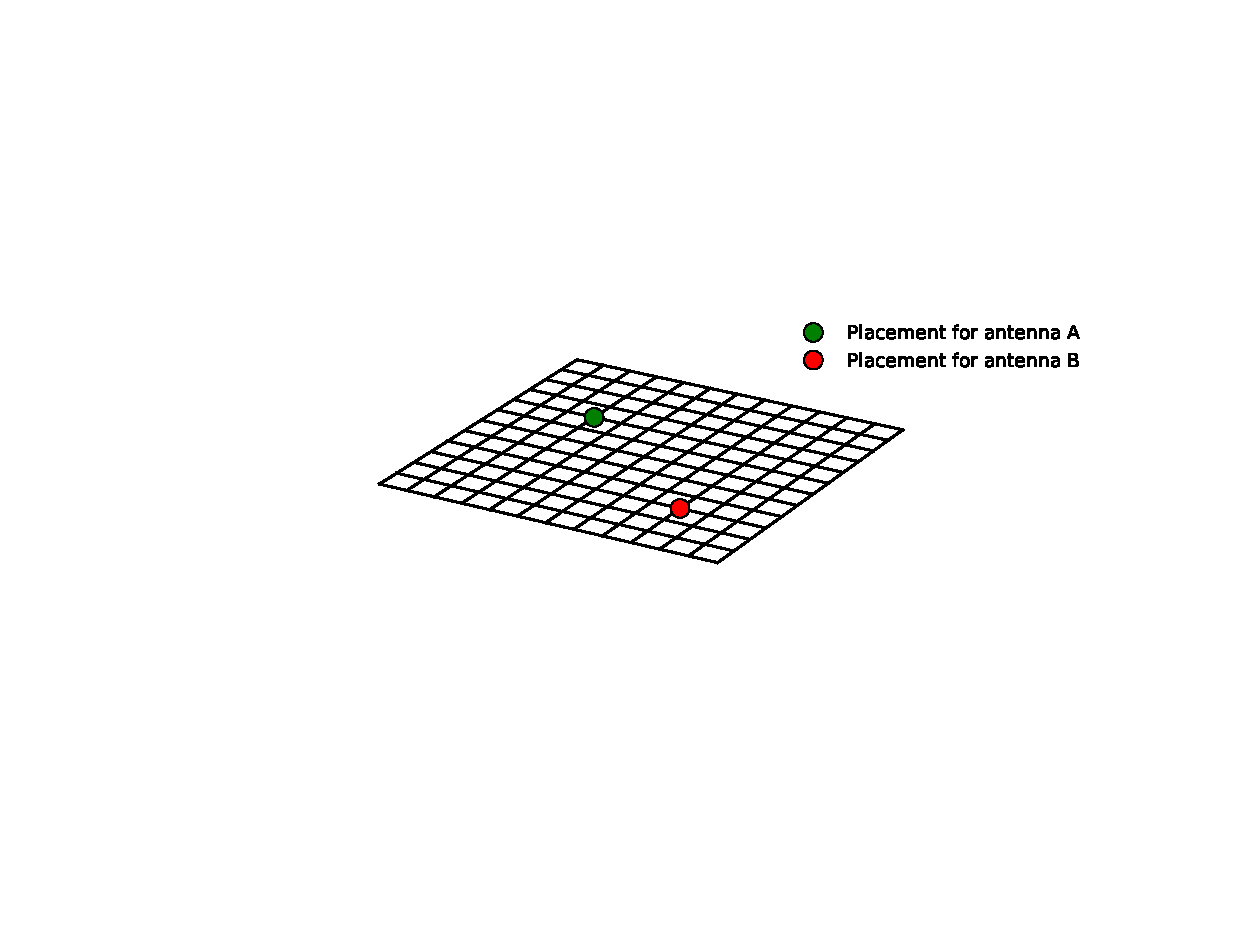
\includegraphics[trim=175 165 50 135, clip, scale=0.35]{../paper/FIG/tc1_mut1}
                $\bigcdot~\bigcdot~\bigcdot$
                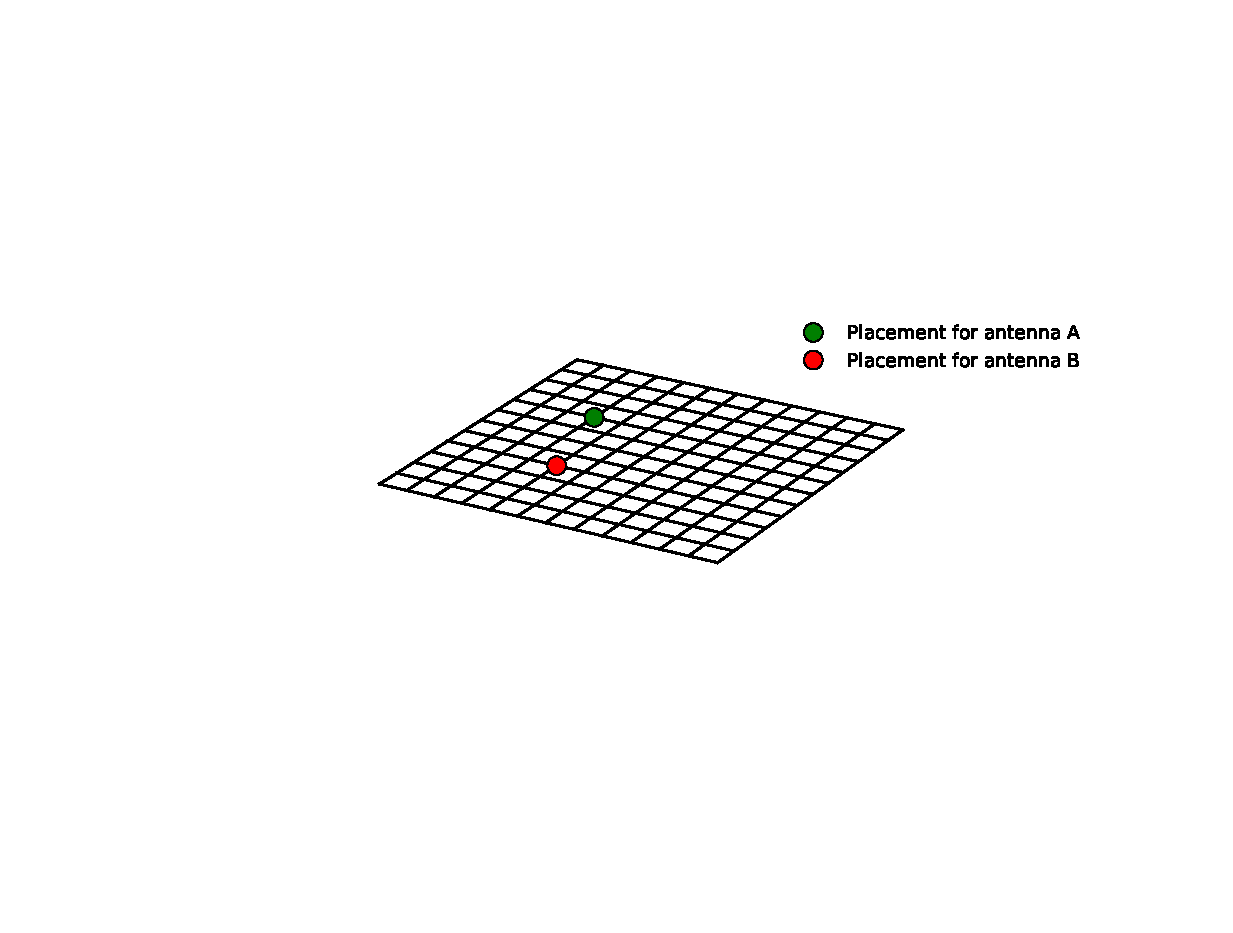
\includegraphics[trim=125 165 50 135, clip, scale=0.35]{../paper/FIG/tc1_mut3}
            }
    \end{itemize}
\end{frame}

\begin{frame}[t]{Mutation Operator}
    \begin{enumerate}
        \item Given an individual, select an antenna uniformly at random, say antenna B:\par
            \begin{minipage}[t]{\linewidth}
                \centering
                \adjustbox{valign=t}{%
                    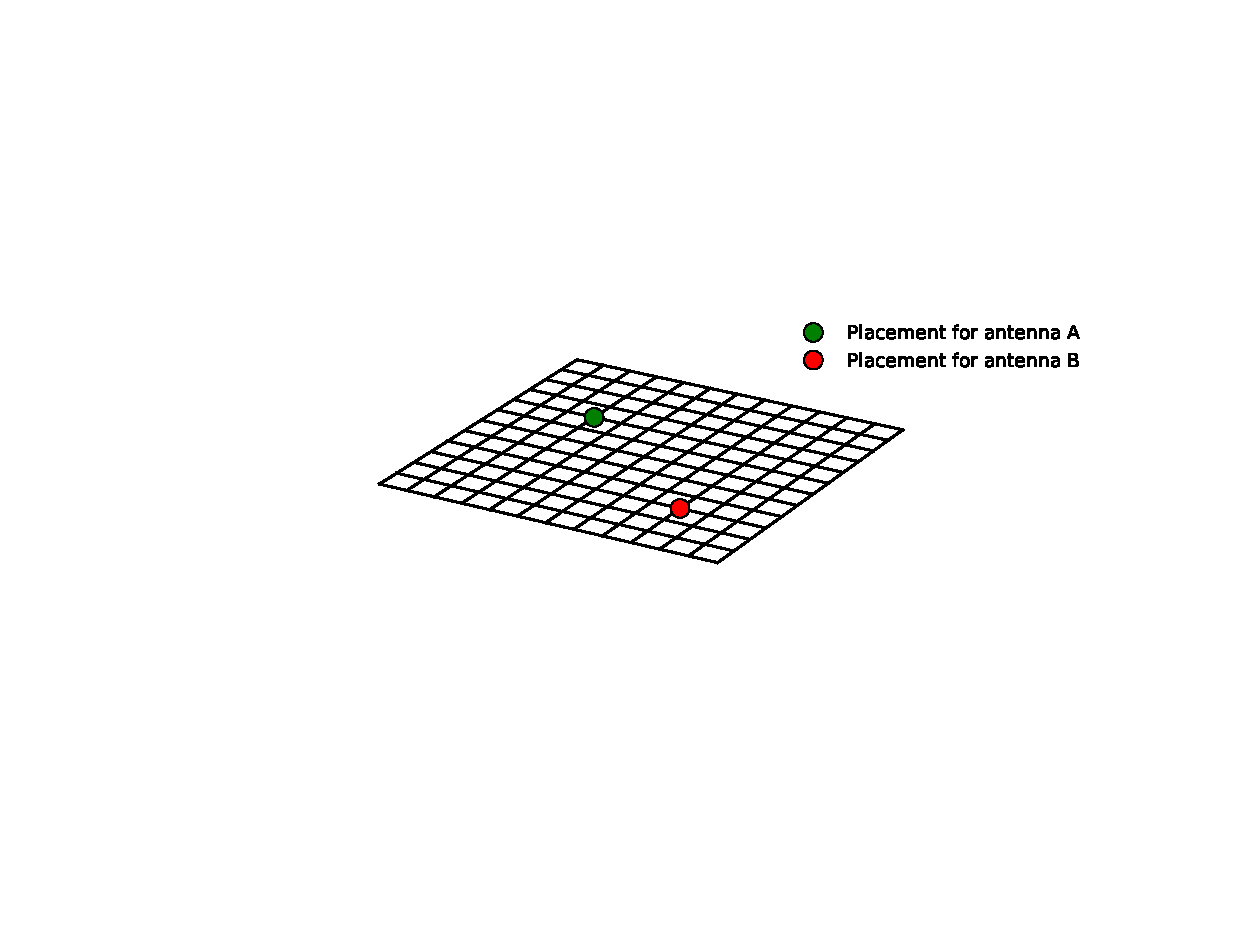
\includegraphics[trim=175 165 50 145, clip, scale=0.35]{../paper/FIG/tc1_mut1}
                }
            \end{minipage}
        \item Select uniformly at random from other allowable placements of antenna $B$: \par
            \begin{minipage}[t]{\linewidth}
                \centering
                \adjustbox{valign=t}{%
                    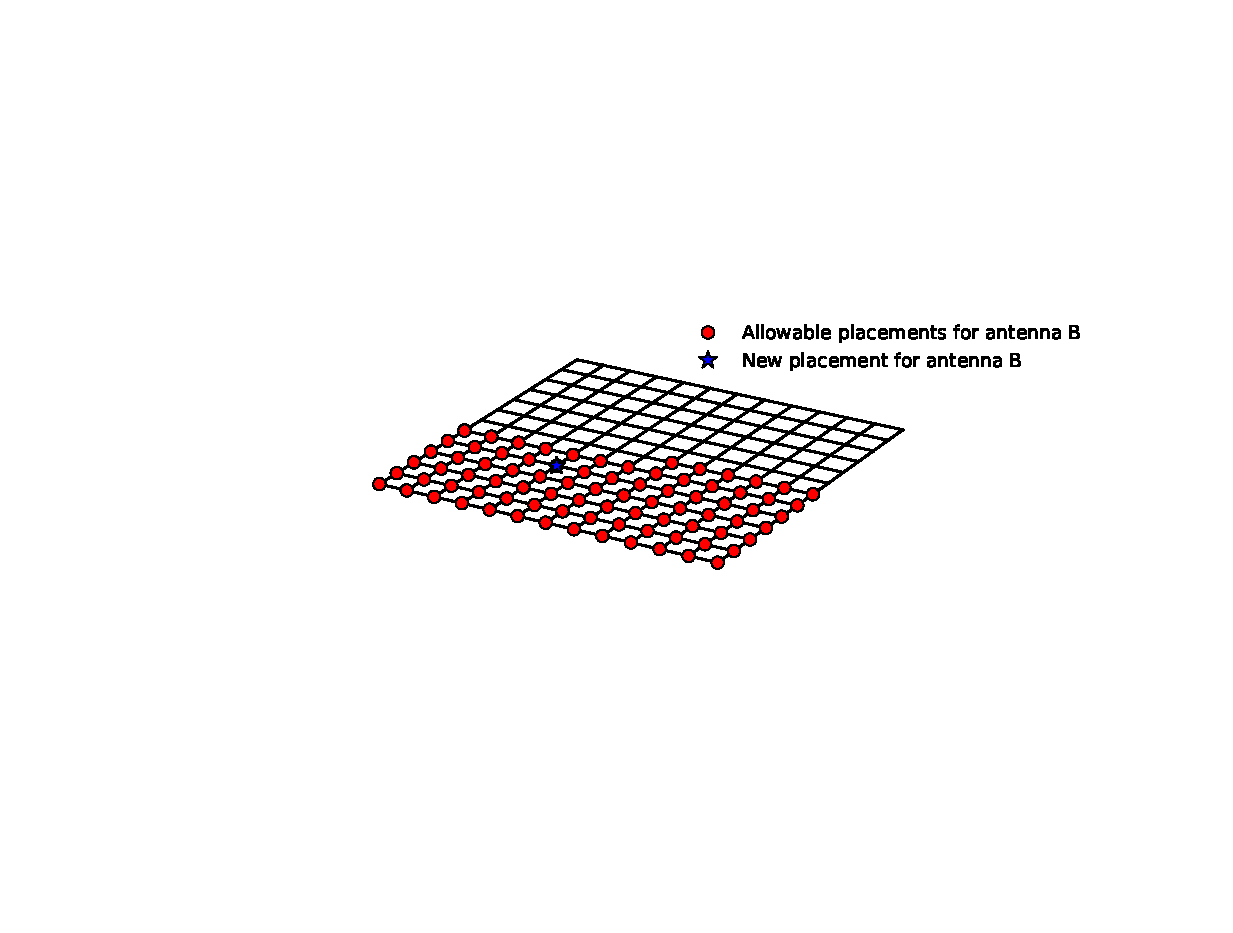
\includegraphics[trim=125 165 50 145, clip, scale=0.35]{../paper/FIG/tc1_mut2}
                }
            \end{minipage}
        \item Change position for antenna B in individual, whereas antenna A's position remains same:\par
            \begin{minipage}[t]{\linewidth}
                \centering
                \adjustbox{valign=t}{%
                    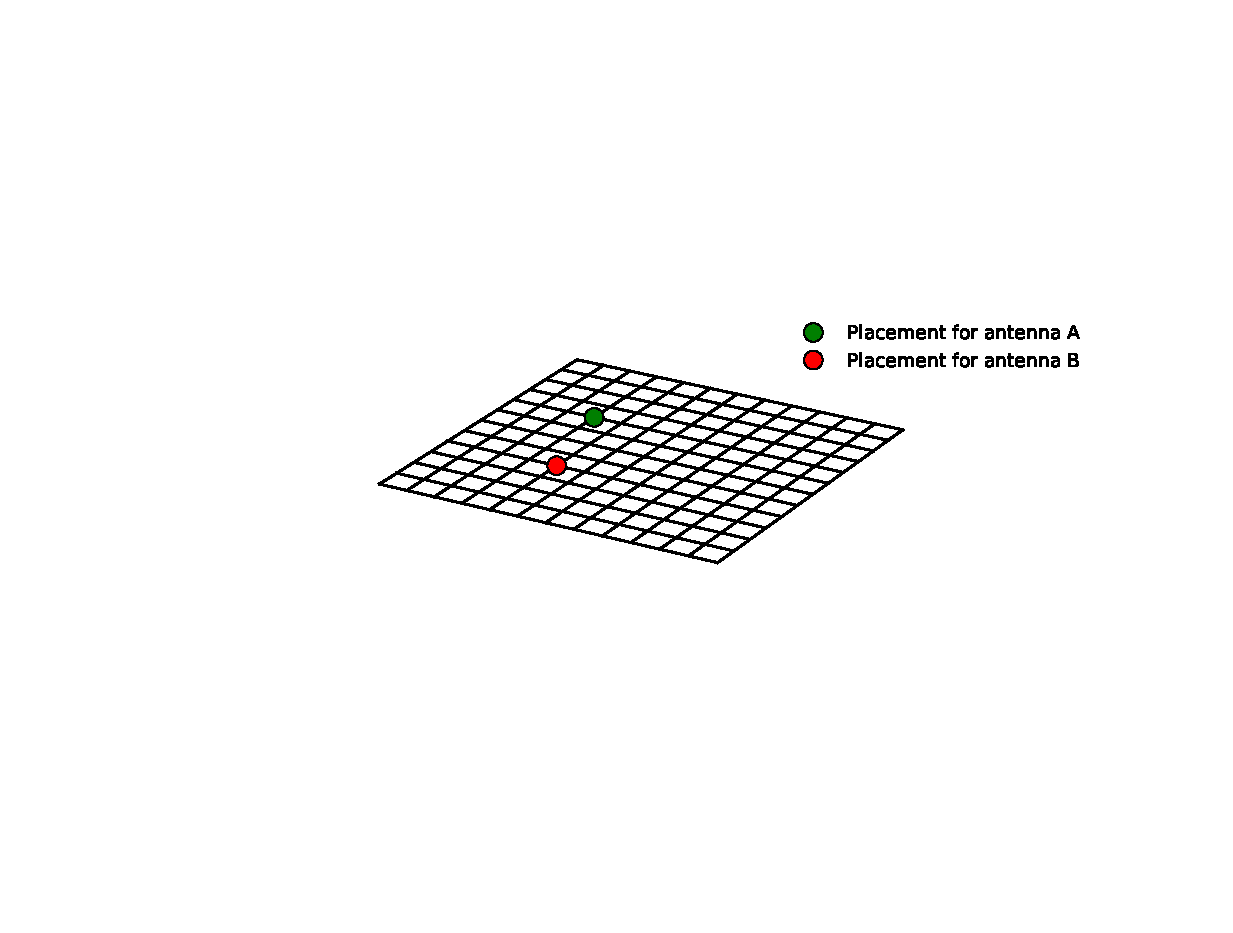
\includegraphics[trim=125 165 50 145, clip, scale=0.35]{../paper/FIG/tc1_mut3}
                }
            \end{minipage}
    \end{enumerate}
\end{frame}

\begin{frame}[t]{Crossover Operator}
    \begin{enumerate}
        \item Select two individuals from population:\par
            \begin{minipage}[t]{\linewidth}
                \centering
                \adjustbox{valign=t}{%
                    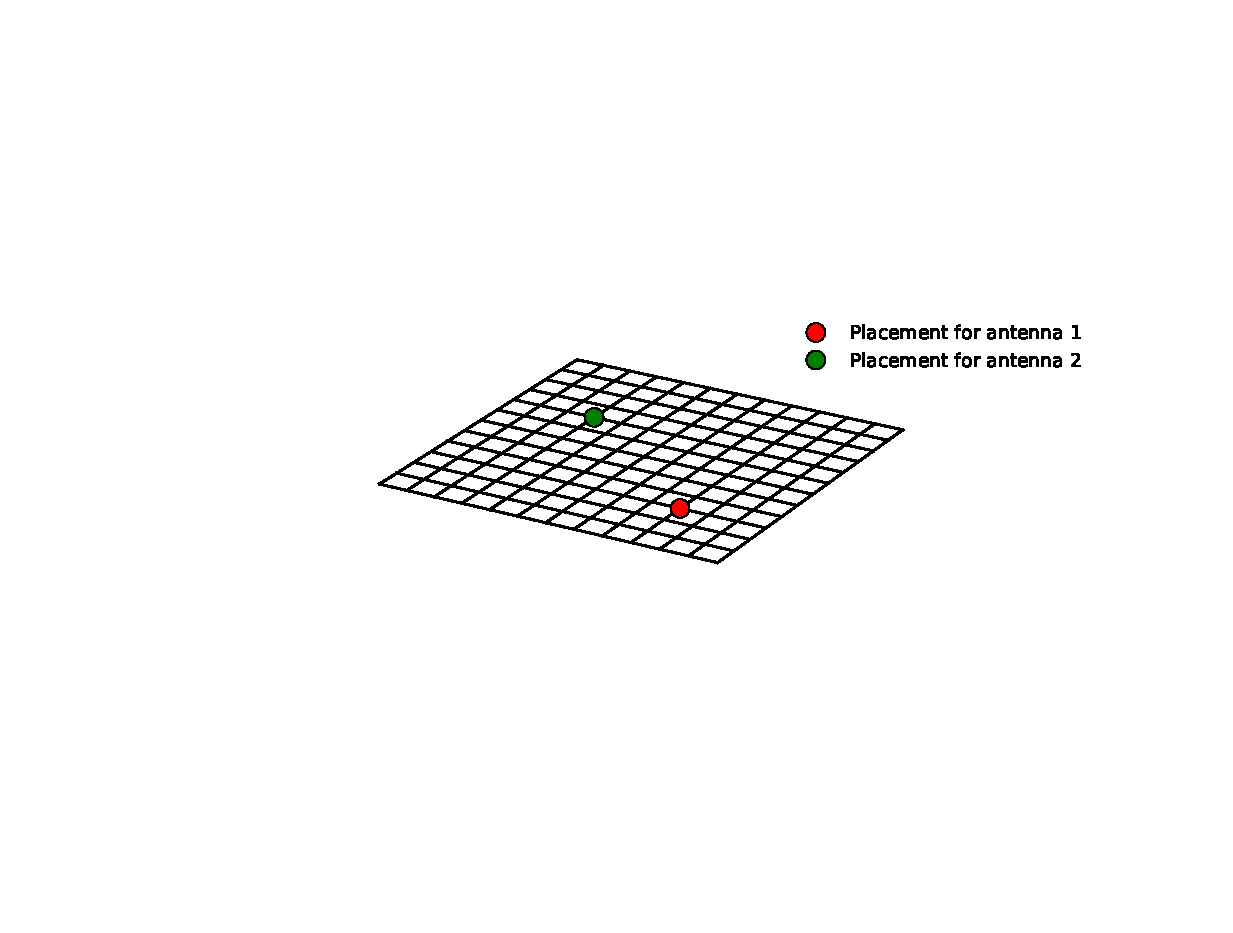
\includegraphics[trim=175 165 50 135, clip, scale=0.35]{../paper/FIG/tc1_reco1}
                    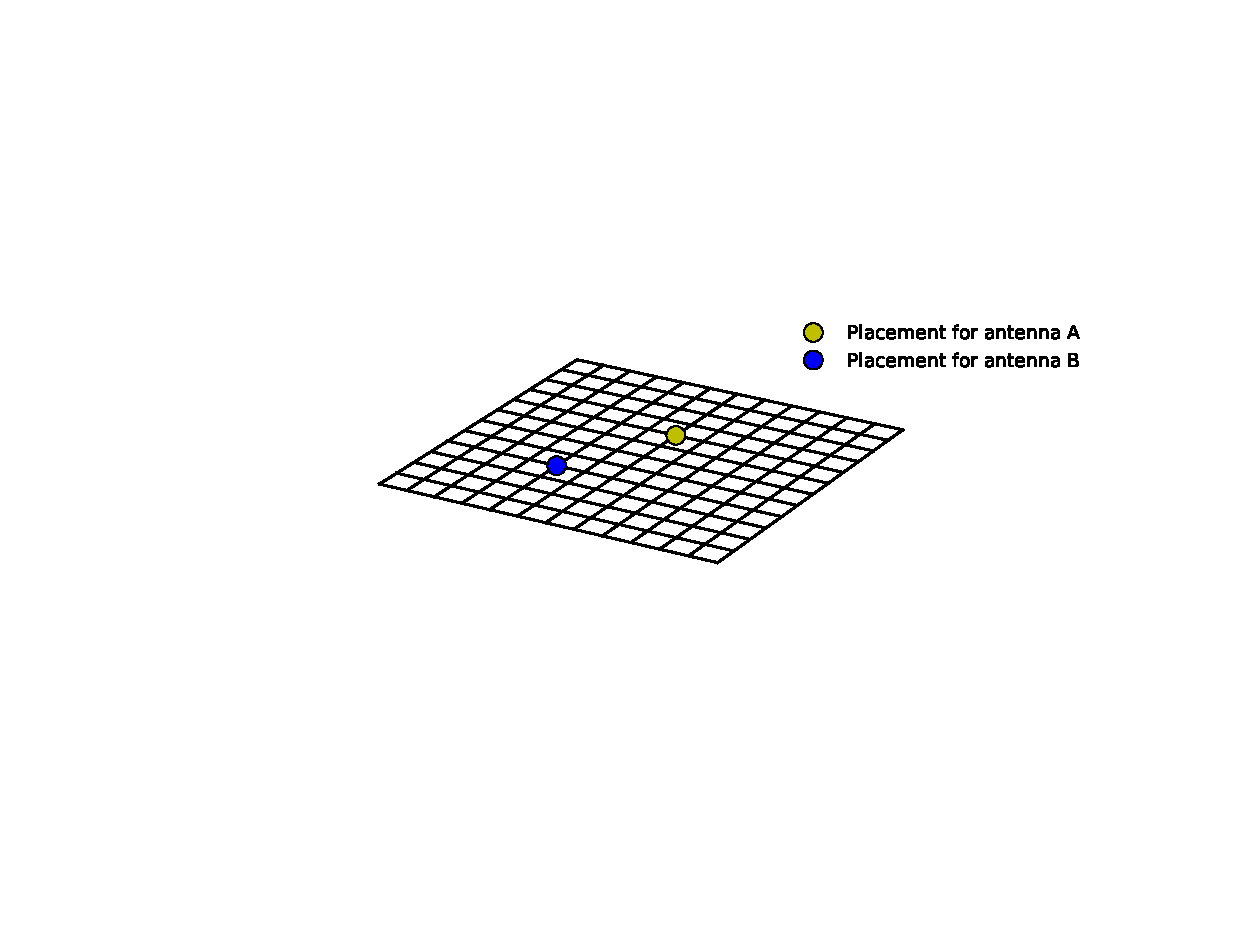
\includegraphics[trim=175 165 50 135, clip, scale=0.35]{../paper/FIG/tc1_reco2}
                }
            \end{minipage}
        \item Select a crossover point, and swap placements prior to the point: \par
            \begin{minipage}[t]{\linewidth}
                \centering
                \adjustbox{valign=t}{%
                    \begin{tabular}{ll:l}
                        $\text{ind}_1:$&$\textcolor{drkgreen}{A}$ & $\textcolor{red}{B}$ \\
                        &\makebox[\widthof{A\_1}][l]{$\downarrow~\uparrow$} &\\
                        $\text{ind}_2:$&$\textcolor{aureolin}{A}$ & $\textcolor{blue}{B}$ \\
                    \end{tabular}
                }
            \end{minipage}
        \item Two new offsprings created:\par
            \begin{minipage}[t]{\linewidth}
                \centering
                \adjustbox{valign=t}{%
                    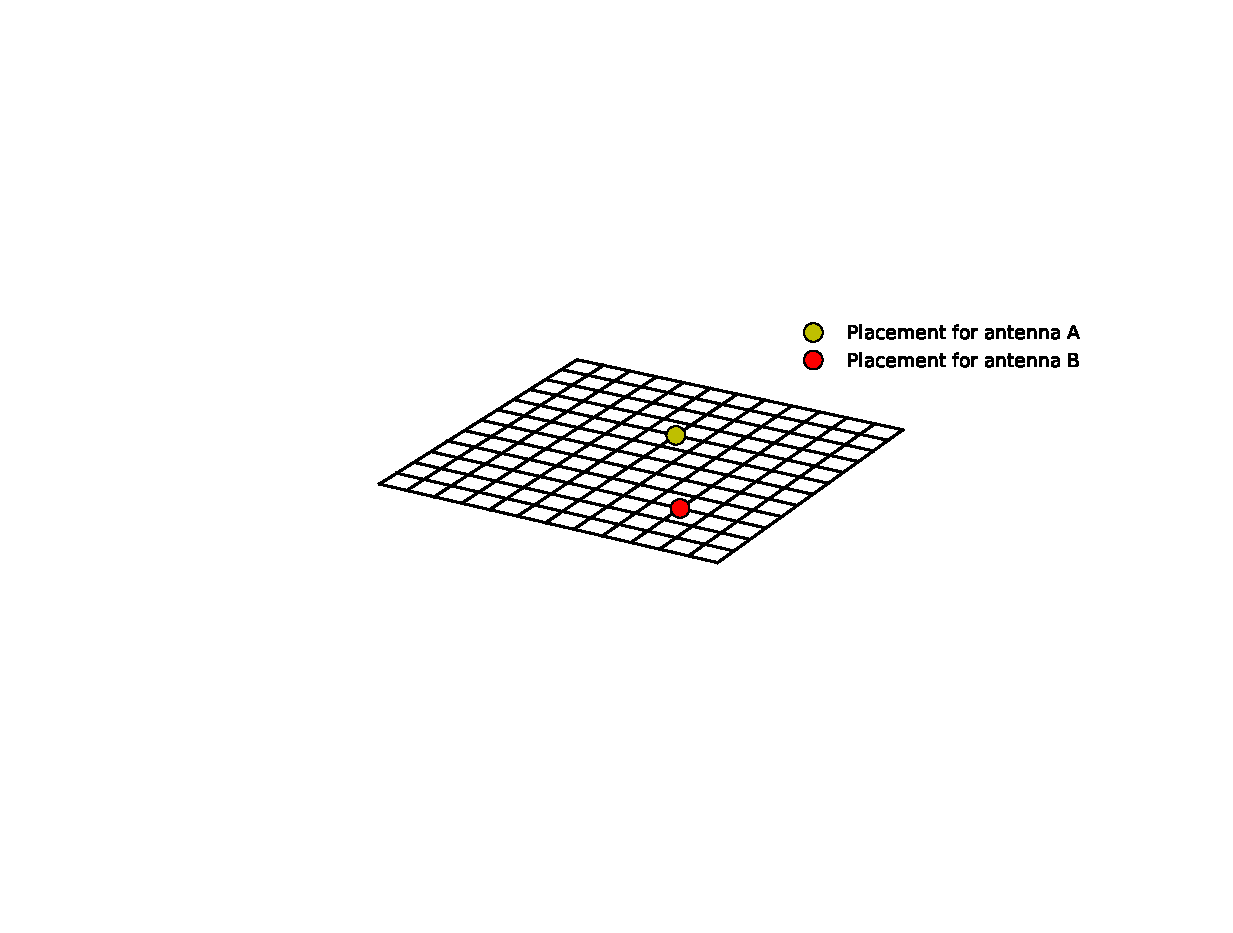
\includegraphics[trim=175 165 50 135, clip, scale=0.35]{../paper/FIG/tc1_reco3}
                    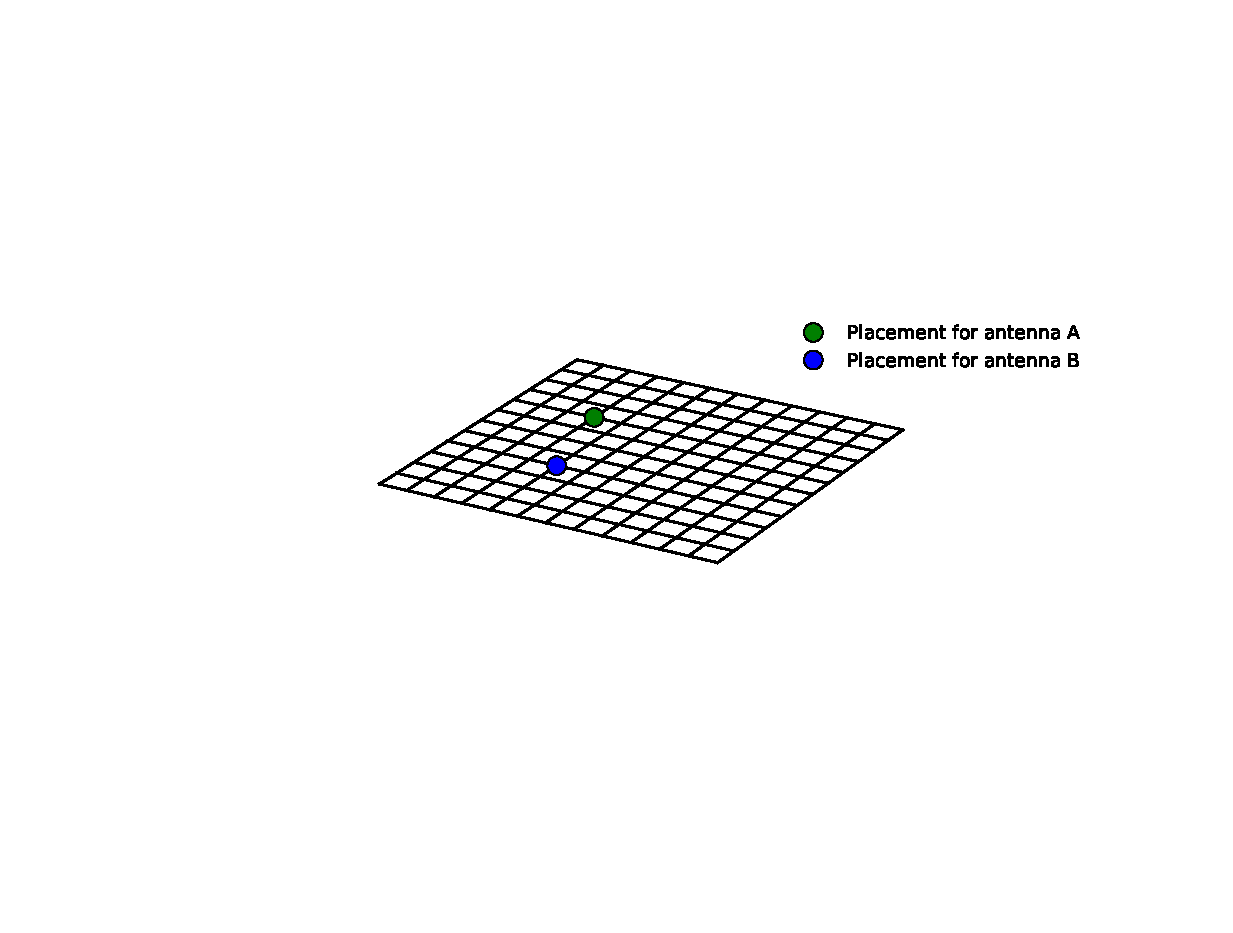
\includegraphics[trim=175 165 50 135, clip, scale=0.35]{../paper/FIG/tc1_reco4}
                }
            \end{minipage}
    \end{enumerate}
\end{frame}

\begin{frame}[t]{Stochastic Algorithms}
    We will consider algorithms which are based on randomization principle:
    \vspace{10px}
\begin{itemize}\itemsep1.5em
        \item Operate on a population of individuals:
        \begin{itemize}\itemsep1.5em
                    \vspace*{1em}
                \item[1.] \textbf{Genetic Algorithm}
                \item[2.] \textbf{Evolutionary Strategy}
            \end{itemize}
        \item Operate on a single individual:
        \begin{itemize}\itemsep1.5em
                    \vspace*{1em}
                \item[3.] \textbf{Simulated Annealing }
                \item[4.] \textbf{Hill Climbing }
    \end{itemize}
    \end{itemize}
\end{frame}


\begin{frame}{\null}
    \begin{tcolorbox}[colback=green!5]
        \centering
        Question: Why use stochastic algorithms?
    \end{tcolorbox}
\end{frame}

\begin{frame}[t]{Fitness Plot}
    \begin{figure}
        \vspace*{-0.35cm}
        \centering
        \includegraphics[scale=0.4]{../paper/FIG/tc1_ss}
        \caption*{Search space for one of the test cases evaluated. There are multiple local minimas which makes convergence difficult. z-axis is the combined fitness $F$}
    \end{figure}
\end{frame}


\begin{frame}{Genetic Algorithm}
    \begin{columns}
        \begin{column}{0.66\linewidth}%added for this algorithm since text wasn't fitting in one slide
            \begin{spacing}{1}
                \fontsize{8}{12}\selectfont
                \setlength{\interspacetitleruled}{0pt}%
                \setlength{\algotitleheightrule}{0pt}%
                \begin{algorithm}[H]
                    Generate initial populaiton $P_0$\;
                    Compute fitness of each individual\;
                    $i \leftarrow 1$ \;
                    \While{$i<gen_{max}$} {
                        $P_i \leftarrow \emptyset$ \;
                        \textcolor{red}{Elitism: Copy some percentage of fittest inidividuals to $P_i$} \;
                        \For{(population\_size - elites) $/2$ } {
                            Select a pair of individuals  \;
                            \textcolor{red}{Perform $crossover$ with some probability}\;
                             Add new or original pair as it is to $P_i$\;
                        }
                        \textcolor{red}{Apply \textit{mutation} to a fraction of individuals in $P_i$}\;
                        Update $i \leftarrow i + 1$ \;
                    }
                \end{algorithm}
            \end{spacing}
        \end{column}
        \begin{column}{0.3\linewidth}
                \begin{figure}
                    \only<1>{\centerline{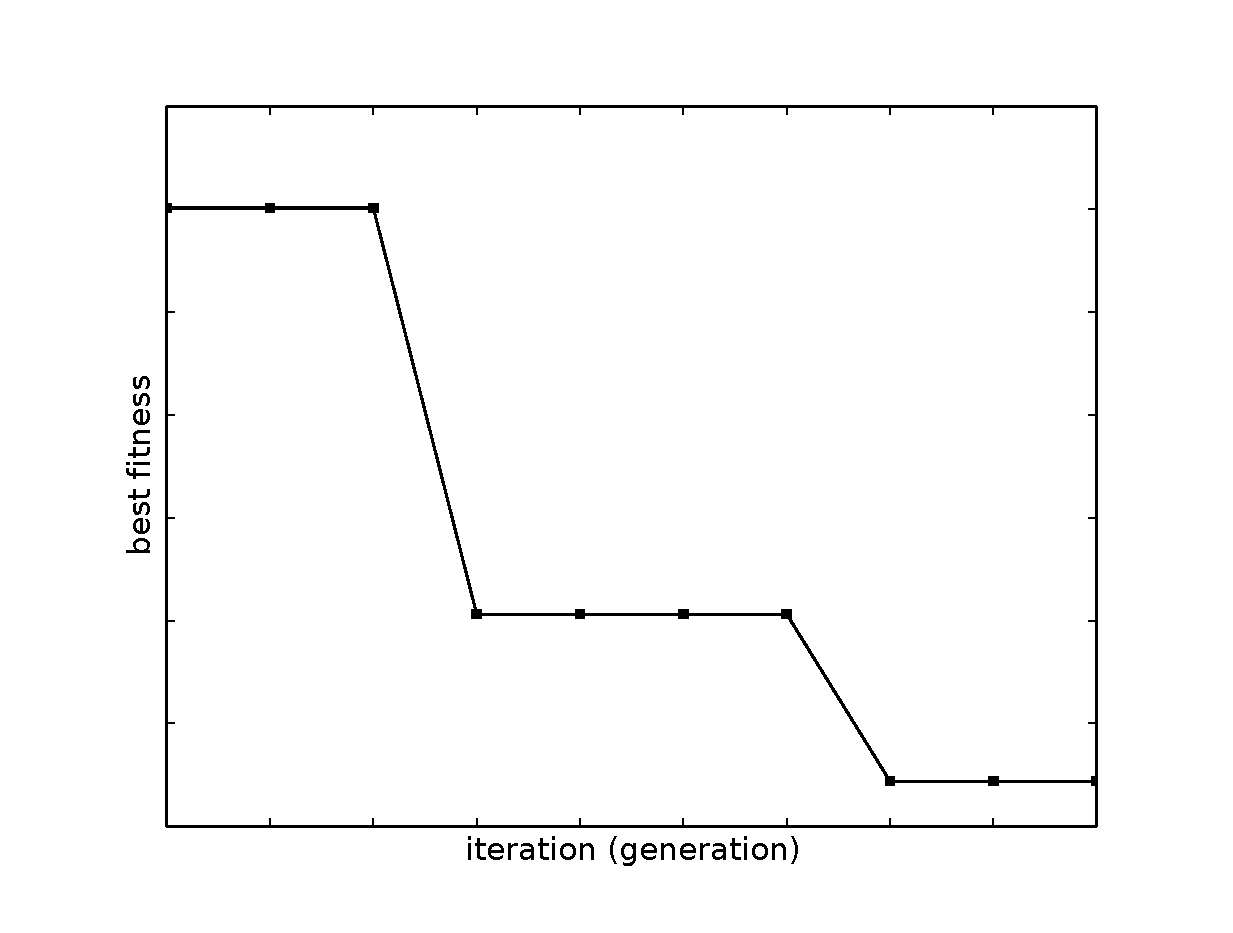
\includegraphics[width=4cm]{../paper/FIG/algo_ga}}
                    \caption*{\tiny \textbf{Example:} Progress of GA applied fitness minimization problem. Each point shows the fitness of the best individual over iterations.}}
                    \only<2>{\centerline{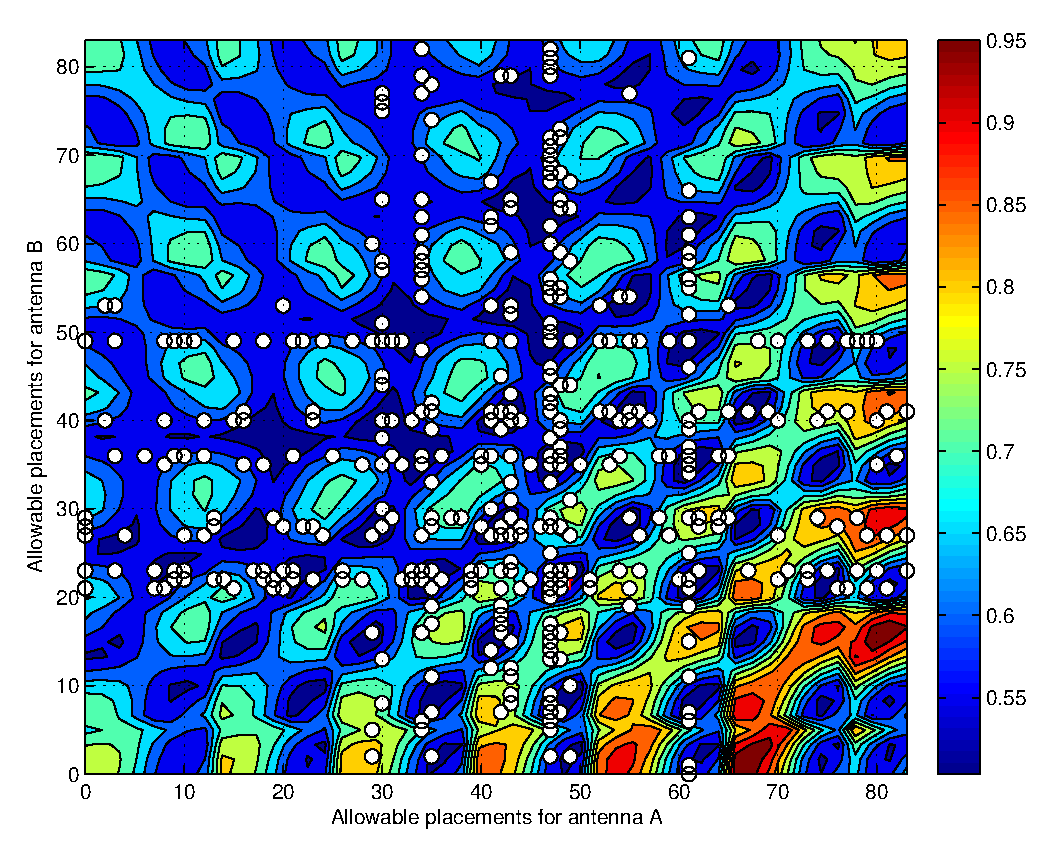
\includegraphics[width=4cm]{../paper/FIG/tc1_ga_anim}}
                    \caption*{\tiny Fitness of population shown with \tikz\draw[black,fill=white] (0,0) circle (.3ex); for last iteration over the contour plot. Population has less diversity.}}
                \end{figure}
        \end{column}
    \end{columns}
\end{frame}


\begin{frame}{Evolutionary Strategy}
    \begin{columns}
        \begin{column}{0.66\linewidth}
            \begin{spacing}{1.2}
            \fontsize{8}{12}\selectfont
            \setlength{\interspacetitleruled}{0pt}%
            \setlength{\algotitleheightrule}{0pt}%
            \begin{algorithm}[H]
                Generate initial populaiton $P_0$\;
                Compute fitness of each individual\;
                $i \leftarrow 1$ \;
                \While{$i<gen_{max}$} {
                    $P_i \leftarrow \emptyset$ \;
                    \textcolor{red}{Apply $mutation$ operator multiple times to each individual in $P_{i-1}$ to create offsprings} \;
                    Compute fitness for all offsprings \;
                    \textcolor{red}{Copy a fraction of $P_{i-1}$ individuals ordered by fitness into $P_i$} \;
                    Update $i \leftarrow i+1$
                }
            \end{algorithm}
        \end{spacing}
        \end{column}
        \begin{column}{0.3\linewidth}
                \begin{figure}
                    \only<1>{\centerline{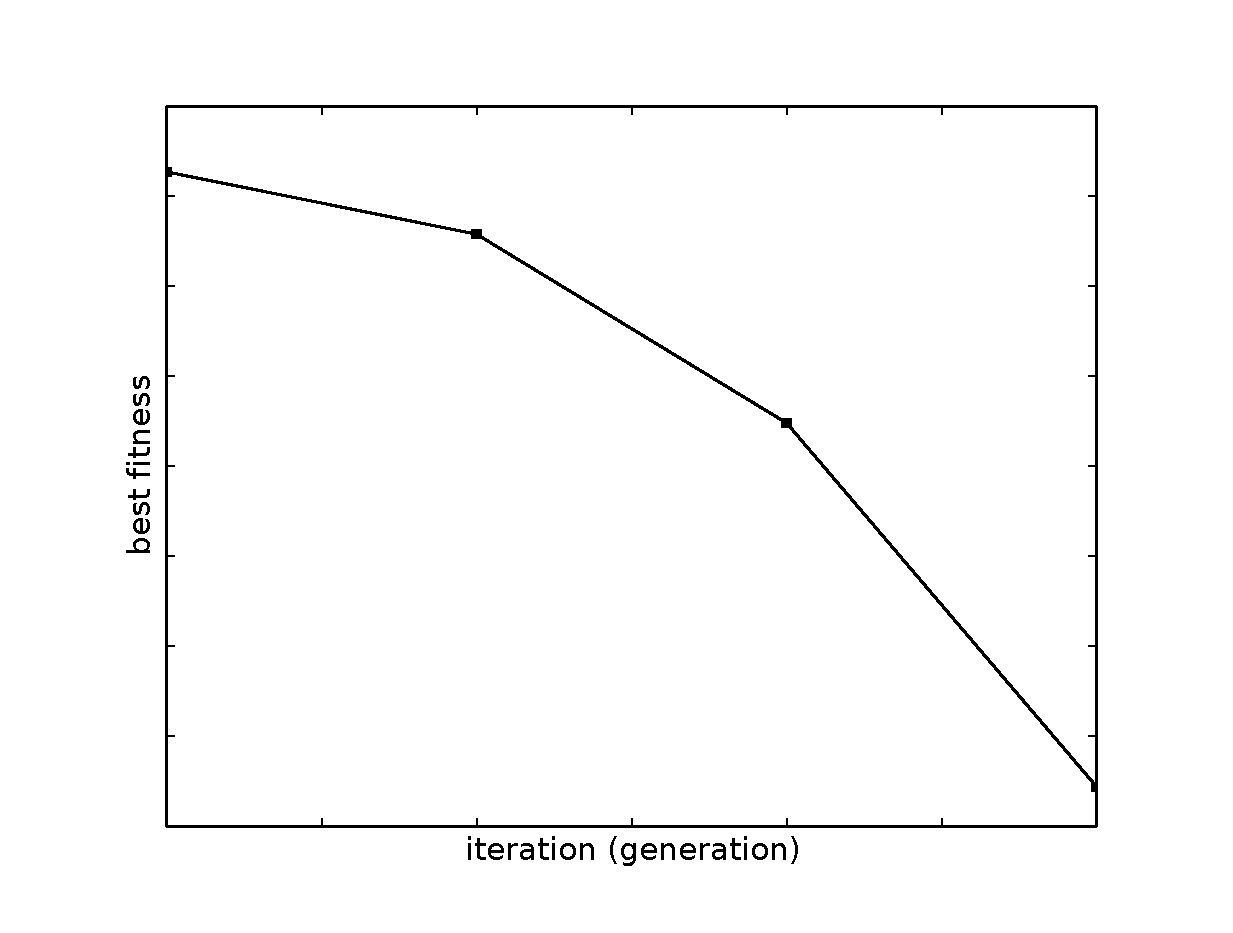
\includegraphics[width=5cm]{../paper/FIG/algo_es}}
                    \caption*{\tiny \textbf{Example:} Progress of ES applied to fitness minimization problem}}
                    \only<2>{\centerline{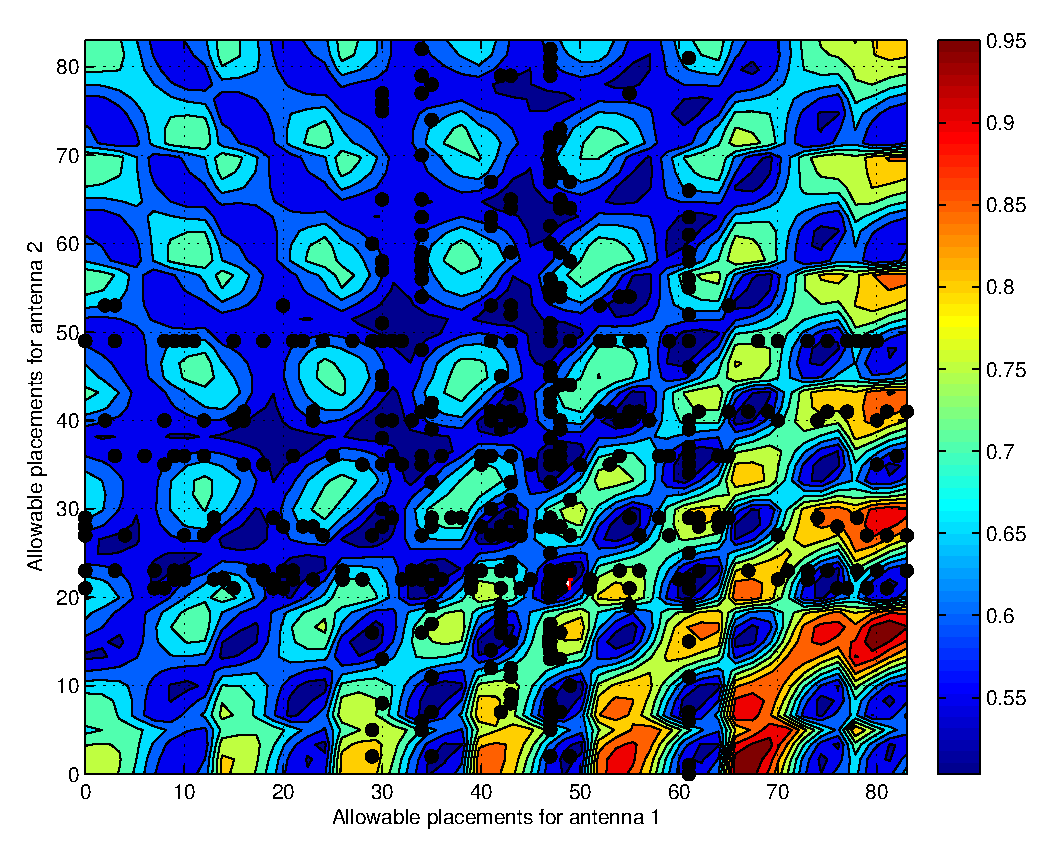
\includegraphics[width=4cm]{../paper/FIG/tc1_es_anim}}
                    \caption*{\tiny Fitness of a population shown with \tikz\draw[black,fill=white] (0,0) circle (.3ex); for last iteration. Greater diversity in comparison to GA\protect\footnotemark}}
                \end{figure}
        \end{column}
    \end{columns}
    \vspace*{-.2cm}
    \only<2->{{\tiny [1] Spears, William M., and Kenneth A. DeJong. "Dining with GAs: operator lunch theorems."}}
\end{frame}

\begin{frame}{Hill Climbing}
    \begin{columns}
        \begin{column}{0.66\linewidth}
            \begin{spacing}{1.5}
            \setlength{\interspacetitleruled}{0pt}%
            \setlength{\algotitleheightrule}{0pt}%
            \fontsize{8}{8}\selectfont
            \begin{algorithm}[H]
                Generate a random inidividual $ind_{curr}$ \;
                Compute fitness of $ind_{curr}$  \;
                $i \leftarrow 1$ \;
                \While{$i<i_{max}$} 
                {
                    Create another individual $ind_{new}$ by $mutation$ of $ind_{curr}$ \; 
                    \If{\textcolor{red}{$fitness(ind_{new}) < fitness(ind_{curr})$}}
                    {
                        \textcolor{red}{$ind_{curr} \leftarrow ind_{new}$}
                    }
                    $i \leftarrow i + 1$
                }
                \label{alg:ap-hc}
            \end{algorithm}
        \end{spacing}
        \end{column}
        \begin{column}{0.3\linewidth}
                \begin{figure}
                    \only<1>{\centerline{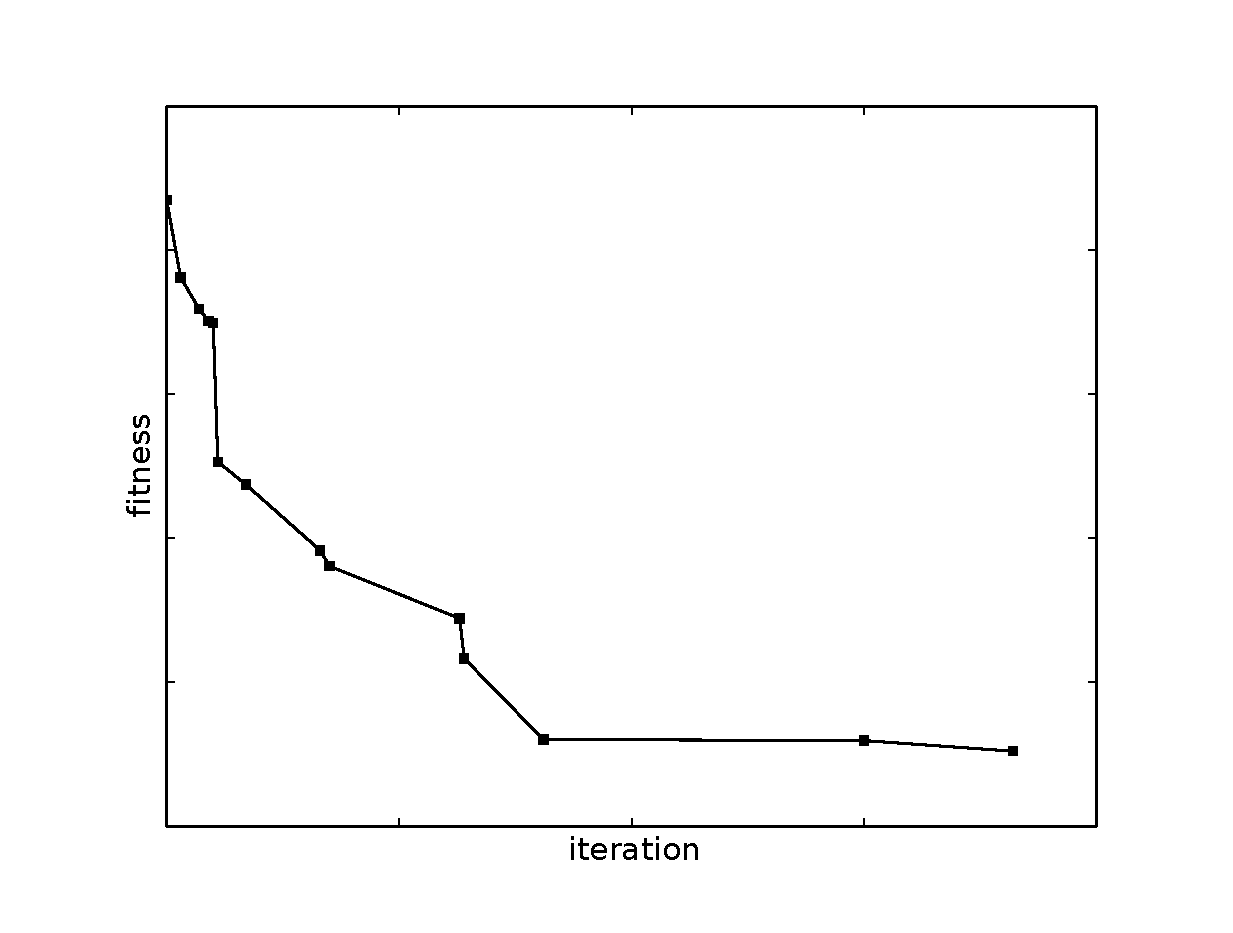
\includegraphics[width=5cm]{../paper/FIG/algo_hc}}
                    \caption*{\tiny \textbf{Example:} Progress of HC applied to fitness minimization problem}}
                    \only<2>{\centerline{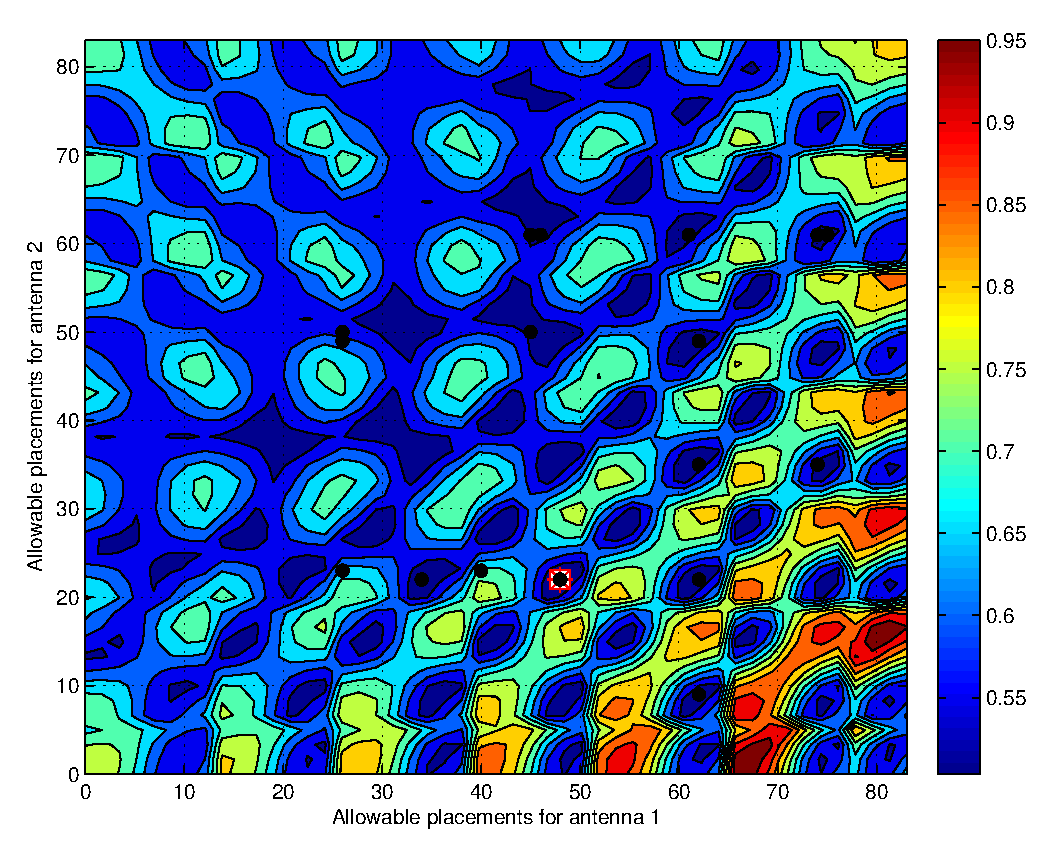
\includegraphics[width=4cm]{../paper/FIG/tc1_hc_anim}}
                    \caption*{\tiny Fitness of $ind_{curr}$ individuals over an entire run shown with \tikz\draw[black,fill=white] (0,0) circle (.3ex);. Search is restricted due to greedy approach to accept only fitter (low fitness) individuals}}
                \end{figure}
        \end{column}
    \end{columns}
\end{frame}

\begin{frame}{Simulated Annealing}
    \begin{columns}
        \begin{column}{0.66\linewidth}
            \setlength{\interspacetitleruled}{0pt}%
            \setlength{\algotitleheightrule}{0pt}%
            \fontsize{8}{8}\selectfont
            \begin{algorithm}[H]
                Generate a random inidividual $ind_{curr}$ \;
                Compute fitness of $ind_{curr}$  \;
                $i \leftarrow 1$ \;
                \While{$i<i_{max}$} 
                {
                    Create another individual $ind_{new}$ by $mutation$ of $ind_{curr}$ \; 
                    \eIf{\textcolor{red}{$fitness(ind_{new}) > fitness(ind_{curr})$}}
                    {
                        \If{$rand() < e^{-\delta f / T}$}
                        {
                            \textcolor{red}{$ind_{curr} \leftarrow ind_{new}$}
                        }
                    }  {$ind_{curr} \leftarrow ind_{new}$}
                    \textcolor{red}{$T \leftarrow T \cdot f_{cooling}$} \;
                    $i \leftarrow i + 1$ \;
                } 
                \label{alg:ap-sa}
            \end{algorithm}
        \end{column}
        \begin{column}{0.3\linewidth}
                    %\only<2>
                    %{
                    %    \movie[height=3.9cm,width=3.9cm]{\tiny Population over generations}{./animation/es.avi}
                    %}
                \begin{figure}
                    \only<1>{\centerline{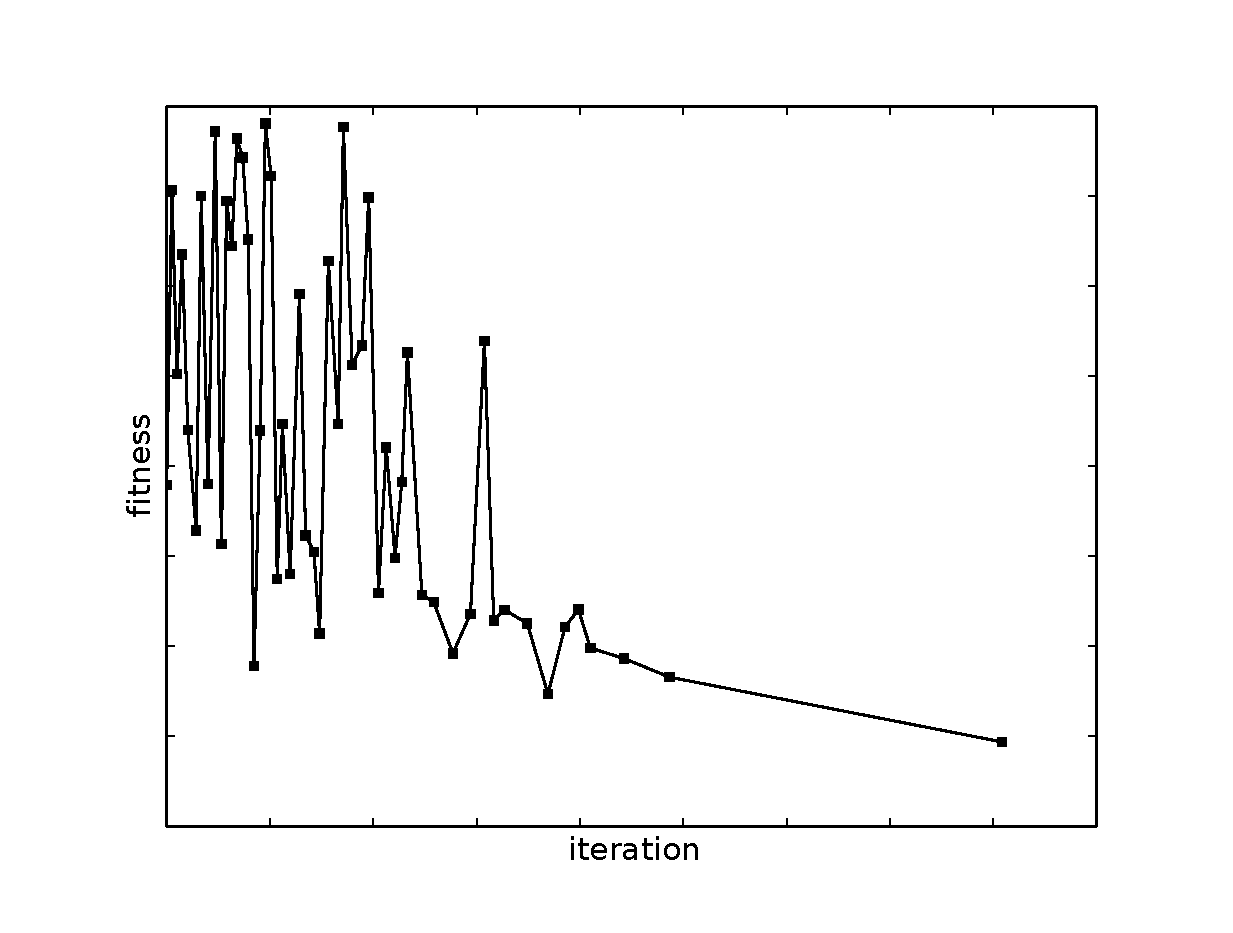
\includegraphics[width=5cm]{../paper/FIG/algo_sa}}
                    \caption*{\tiny \textbf{Example:} Progress of SA applied to fitness minimization problem. As iterations increase, worse individuals with lower delta fitness ($\delta f$) are accepted.}}
                    \only<2>{\centerline{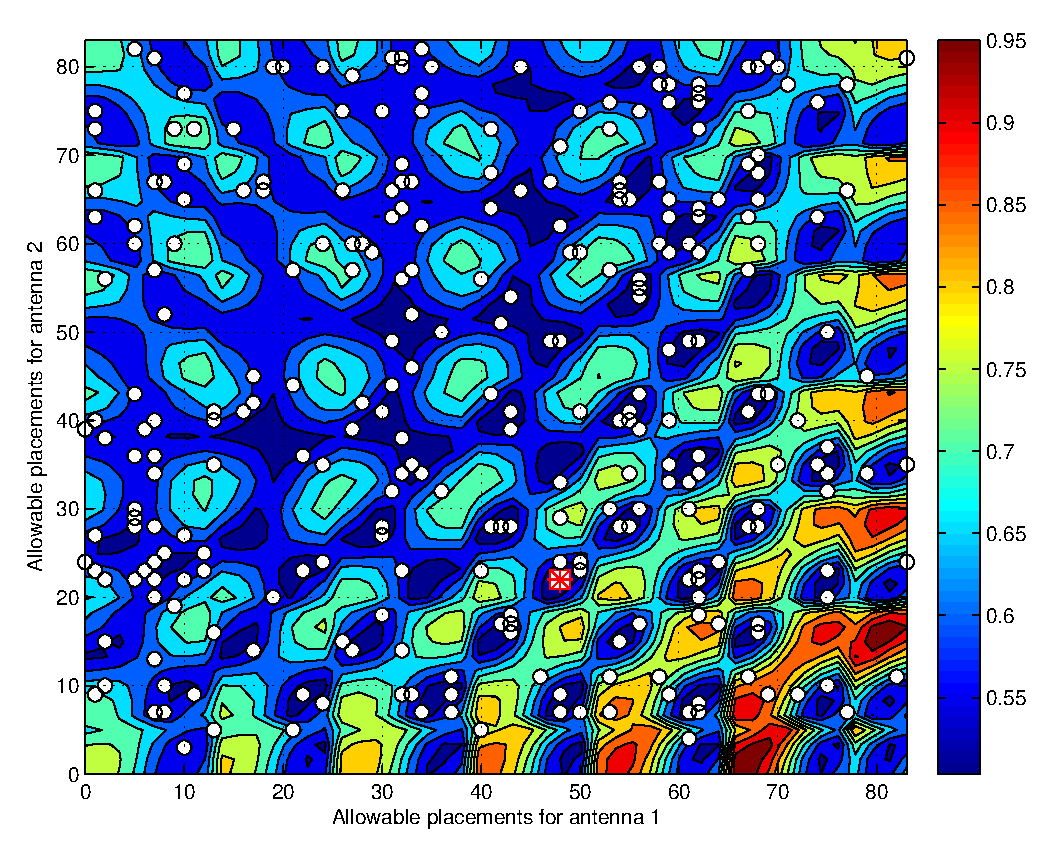
\includegraphics[width=4cm]{../paper/FIG/tc1_sa_anim}}
                    \caption*{\tiny Fitness of $ind_{curr}$ individuals over an entire run shown with \tikz\draw[black,fill=white] (0,0) circle (.3ex);. Search is distributed across the terrain}}
                \end{figure}
        \end{column}
    \end{columns}
\end{frame}

\begin{frame}{\null}
    \begin{tcolorbox}[colback=green!5]
        \centering\Huge
        Part 3: Evaluation of test cases
    \end{tcolorbox}
\end{frame}

\begin{frame}{Experimental Setup}
\begin{enumerate}\itemsep1.2em
        \item We use a popular NEC2 simulator to get fitness parameters 
        \item Evaluated the entire search space using an exhaustive algorithm to find the optimal antenna locations which is not ordinarily possible
        \item Termination criteria was set to be at most $50\%$ evaluations of the search spcae
        \item $1000$ independent runs of each test case against each algorithm with $\alpha = \beta = 1/2$
    \end{enumerate}
    \vspace*{0.5cm}
    \vspace{10mm}
\end{frame}


\begin{frame}{Experiments Test Cases}
    \begin{columns}
        \begin{column}{.5\columnwidth}
            \begin{figure}
                \vspace*{-0.5cm}
                \centering
                \begin{subfigure}{\columnwidth}
                    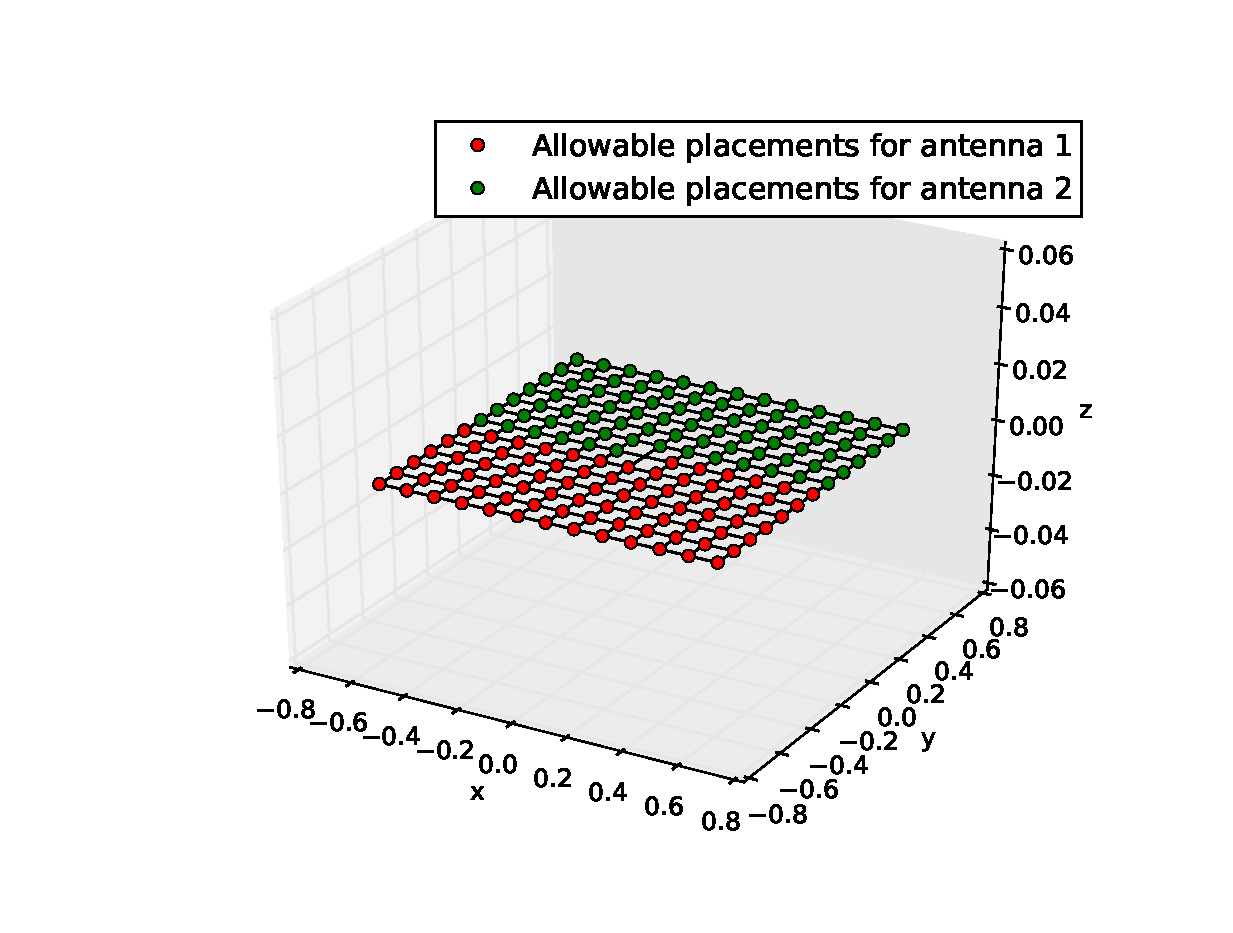
\includegraphics[trim=0 30 0 50, clip,scale=0.25]{../paper/FIG/tc1_figure}%
                    \caption*{\tiny Test Case \#1: search space size of $7056~(84x84)$ allowable placements}%
                \end{subfigure}\hfill\\
                \begin{subfigure}{\columnwidth}
                    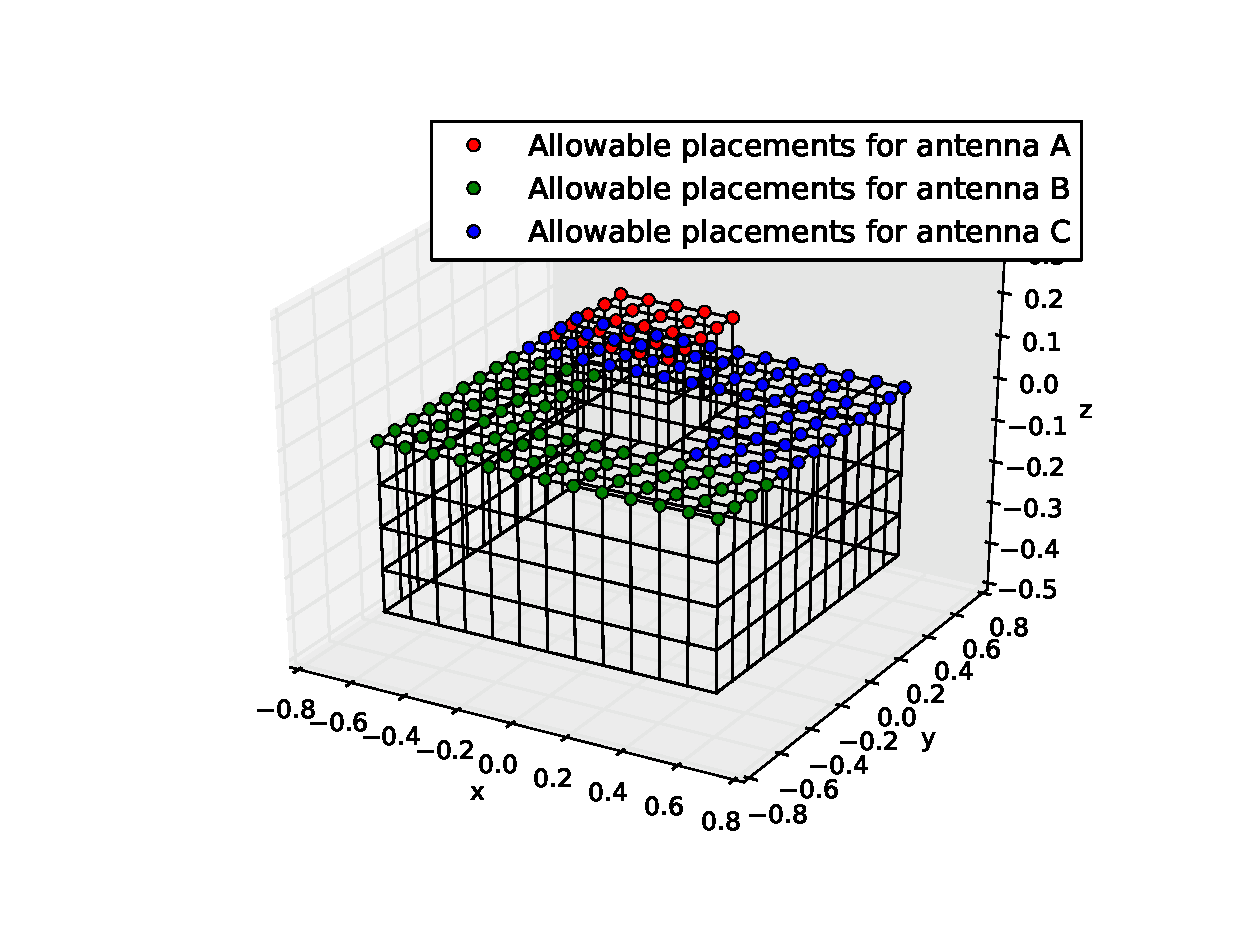
\includegraphics[trim=0 30 0 50, clip, scale=0.25]{../paper/FIG/tc3_figure}%
                    \caption*{\tiny Test Case \#3: search space size of $126025~(71x71x25)$ allowable placements}%
                \end{subfigure}\hfill%
            \end{figure}
        \end{column}
        \begin{column}{.5\columnwidth}
            \begin{figure}
                \vspace{-0.5cm}
                \begin{subfigure}{\columnwidth}
                    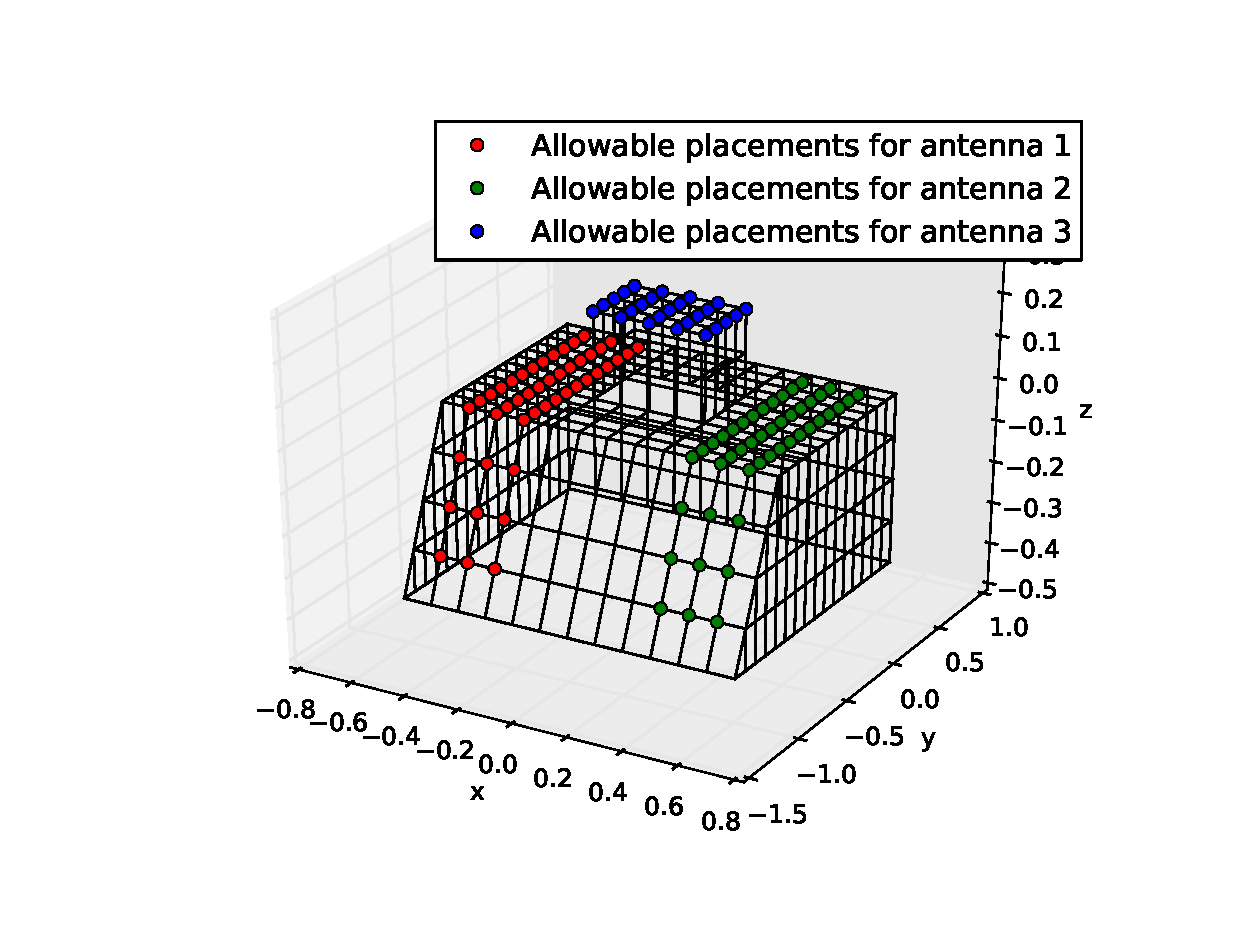
\includegraphics[trim=0 30 0 50, clip, scale=0.25]{../paper/FIG/tc2_figure}%
                    \caption*{\tiny Test Case \#2: search space size of $50625~(45x45x25)$ allowable placements}%
                \end{subfigure}\hfill\\%
                \begin{subfigure}{\columnwidth}
                    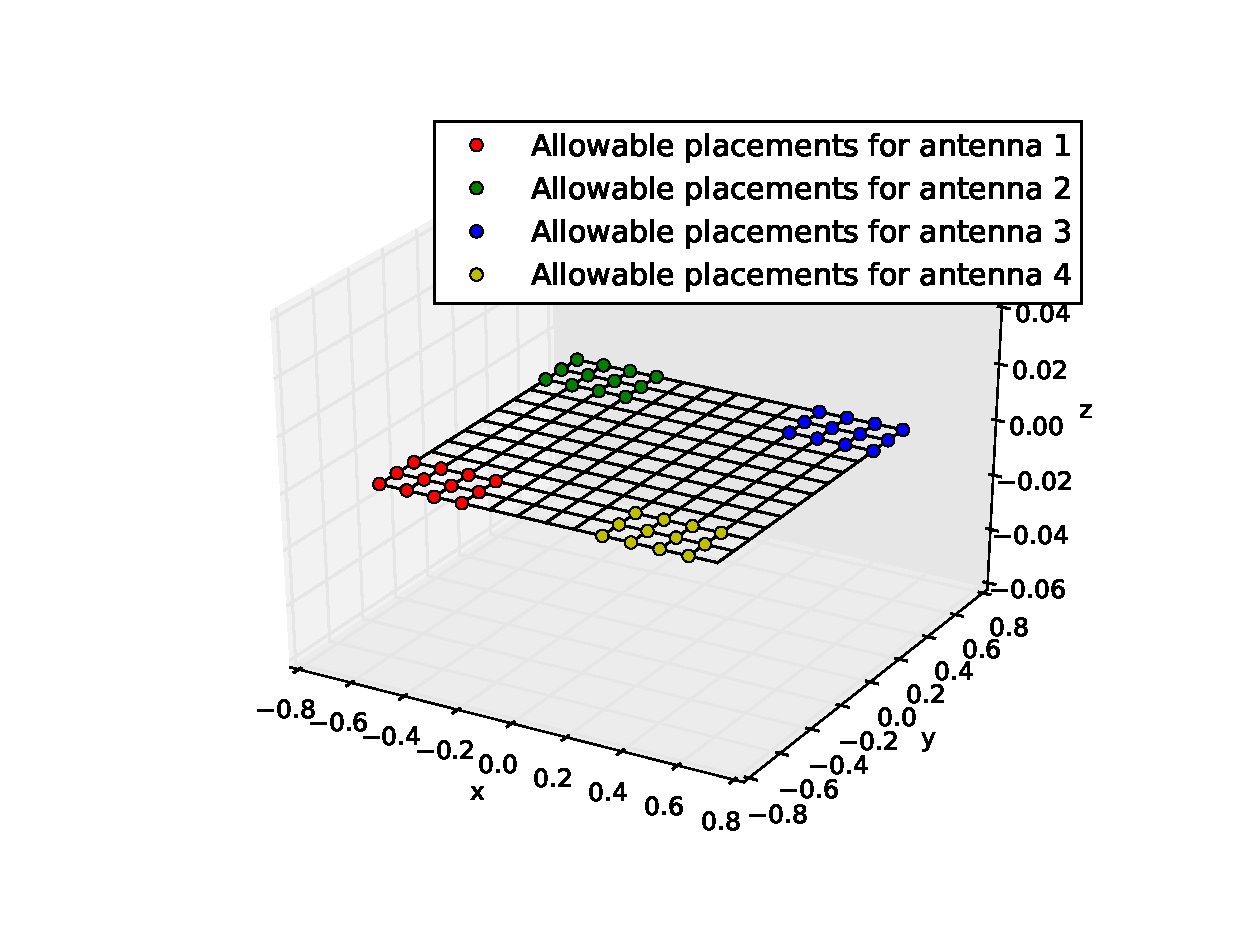
\includegraphics[trim=0 30 0 50, clip, scale=0.25]{../paper/FIG/tc4_figure}%
                    \caption*{\tiny Test Case \#4: search space size of $20736~(12x12x12x12)$ allowable placements}%
                \end{subfigure}\hfill%
            \end{figure}
        \end{column}
    \end{columns}
\end{frame}


\begin{frame}{Results - Test Case 1}
    \begin{columns}
        \begin{column}{\columnwidth}
            {\tiny Sample size = 1000}
            \adjustbox{max width=\columnwidth}{\tiny
                \begin{tabularx}{\columnwidth}{@{}l *4{>{\centering\arraybackslash}X}@{}} 
                    \toprule
                    Algorithm
                    & \multicolumn{2}{c}{\%Evaluations vs. Exhaustive}  
                    & \multicolumn{2}{c}{Best fitness}\\
                    \cmidrule(lr){2-3} \cmidrule(lr){4-5}
                    & Mean & Std. Dev. &  Mean & Std. Dev. \\
                    \midrule
                    ES & 11.88 & 10.48 & \num{0.49865} & \num{0.00009} \\
                    SA & 8.28 & 4.47 & 0.49935 & 0.00163 \\
                    GA & 17.21 & 15.69 & 0.49949 & 0.00182 \\
                    HC & 2.50 & 2.20 & 0.50230 & 0.00501 \\
                    \bottomrule
                \end{tabularx}
            } \vspace*{-0.35cm}
            \begin{figure}
                \centering
                    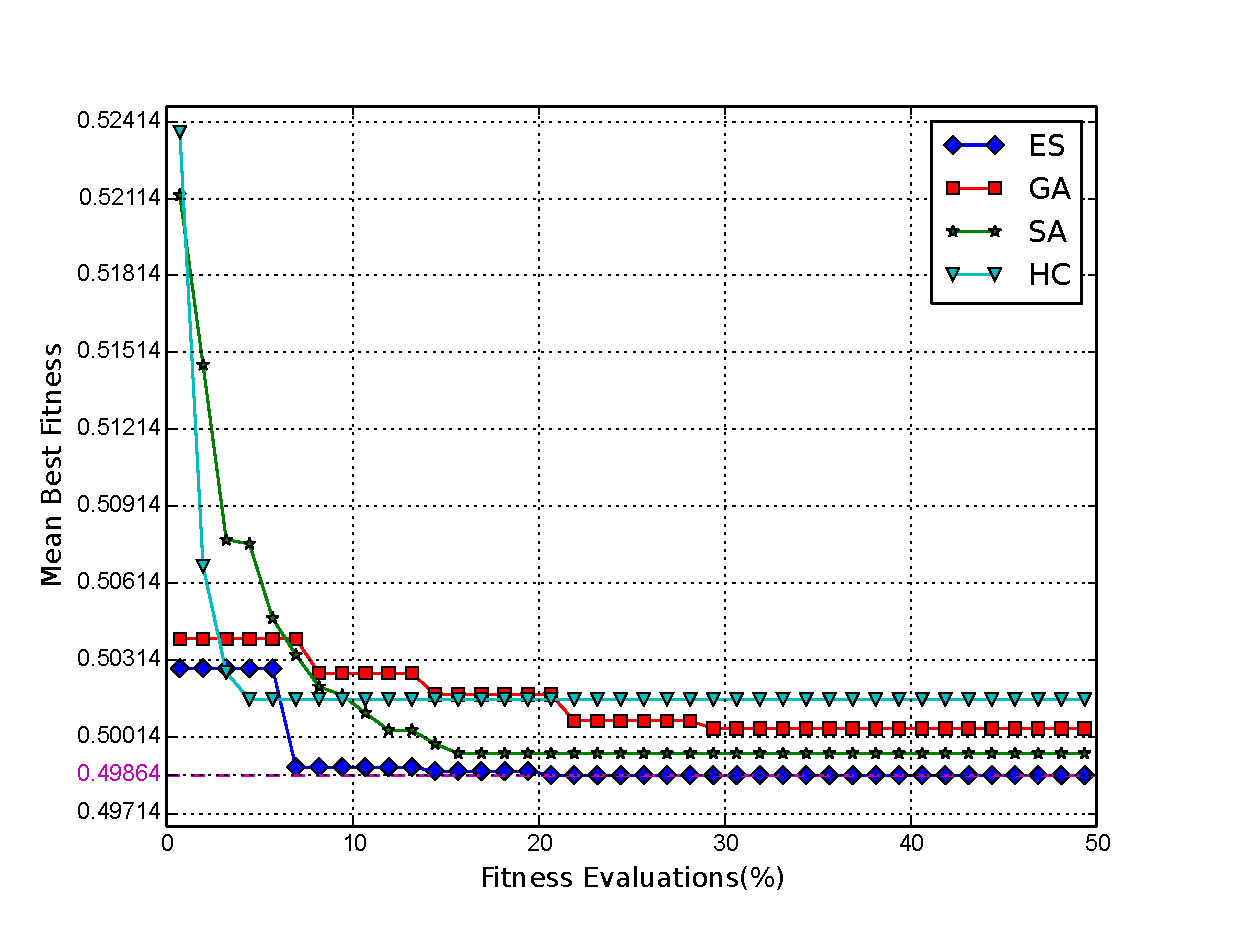
\includegraphics[trim=0 10 0 30,clip,height=5cm,width=8cm]{../paper/FIG/tc1_mf}%
            \end{figure}
        \end{column}
    \end{columns}
\end{frame}

\begin{frame}{Results - Test Case 2}
    \begin{columns}
        \begin{column}{\columnwidth}
            {\tiny Sample size = 1000}
            \adjustbox{max width=\columnwidth}{\tiny
                \begin{tabularx}{\columnwidth}{@{}l *4{>{\centering\arraybackslash}X}@{}} 
                    \toprule
                    Algorithm
                    & \multicolumn{2}{c}{\%Evaluations vs. Exhaustive}  
                    & \multicolumn{2}{c}{Best fitness}\\
                    \cmidrule(lr){2-3} \cmidrule(l){4-5}
                    & Mean & Std. Dev. &  Mean & Std. Dev. \\
                    \midrule
                    ES & 16.08 & 7.72 & 0.49688 & 0.00000 \\
                    SA & 7.96 & 3.33 & 0.49784 & 0.00233 \\
                    GA & 25.98 & 15.51 & 0.50034 & 0.00341 \\
                    HC & 0.40 & 0.31 & 0.51071 & 0.01305 \\
                    \bottomrule
                \end{tabularx}
            } \vspace*{-0.35cm}
            \begin{figure}
                \centering
                    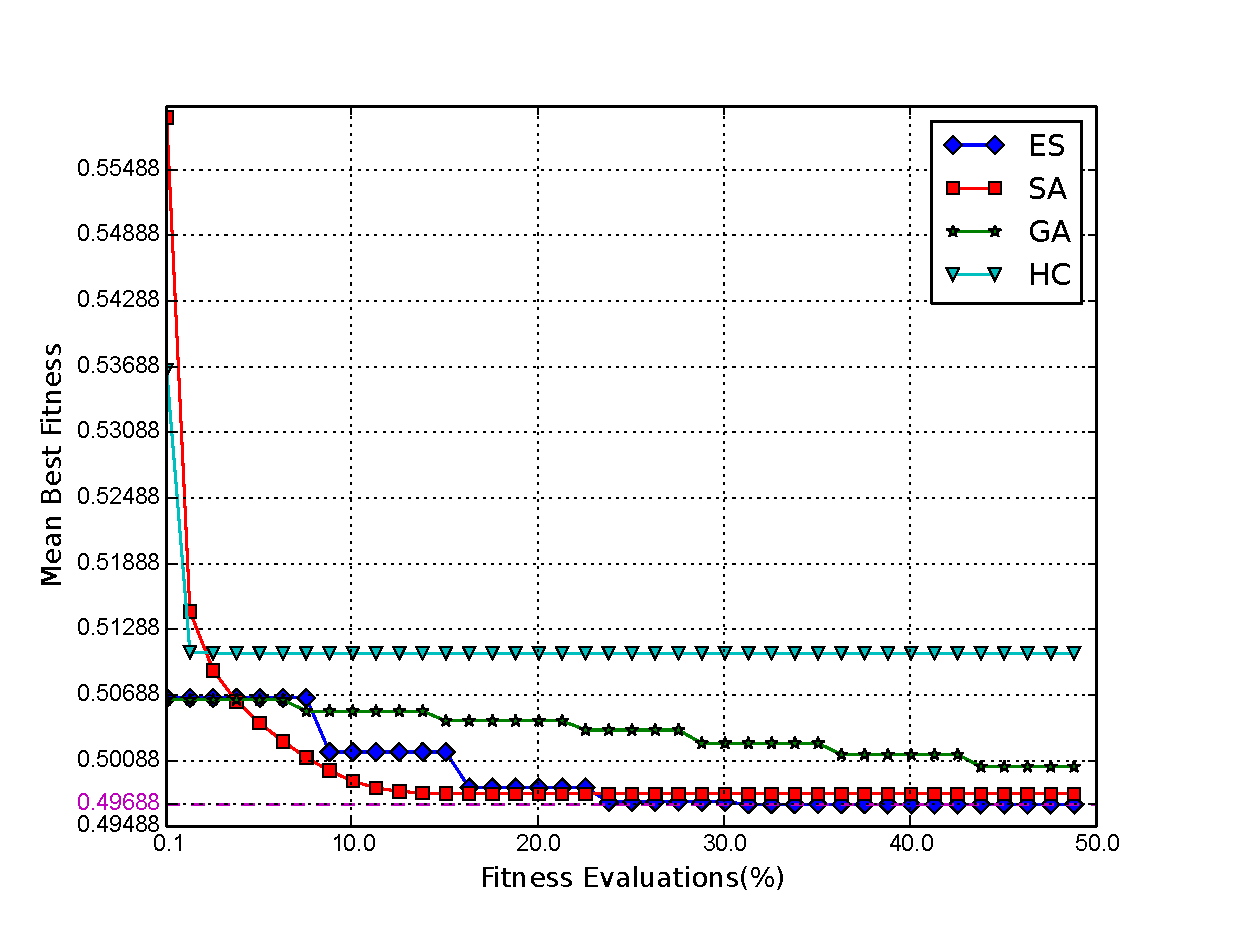
\includegraphics[trim=0 10 0 30,clip,height=5cm,width=8cm]{../paper/FIG/tc2_mf}%
            \end{figure}
        \end{column}
    \end{columns}
\end{frame}


\begin{frame}{Results - Test Case 3}
    \begin{columns}
        \begin{column}{\columnwidth}
            {\tiny Sample size = 1000}
            \adjustbox{max width=\columnwidth}{\tiny
                \begin{tabularx}{\columnwidth}{@{}l *4{>{\centering\arraybackslash}X}@{}} 
                    \toprule
                    Algorithm
                    & \multicolumn{2}{c}{\%Evaluations vs. Exhaustive}  
                    & \multicolumn{2}{c}{Best fitness}\\
                    \cmidrule(lr){2-3} \cmidrule(l){4-5}
                    & Mean & Std. Dev. &  Mean & Std. Dev. \\
                    \midrule
                    ES & 11.04 & 6.72 & 0.49747 & 0.00000 \\
                    SA & 19.61 & 11.16 & 0.49747 & 0.00003 \\
                    GA & 23.05 & 16.25 & 0.49770 & 0.00038 \\
                    HC & 0.21 & 0.17 & 0.49890 & 0.00182 \\
                    \bottomrule
                \end{tabularx}
            } \vspace*{-0.35cm}
            \begin{figure}
                \centering
                    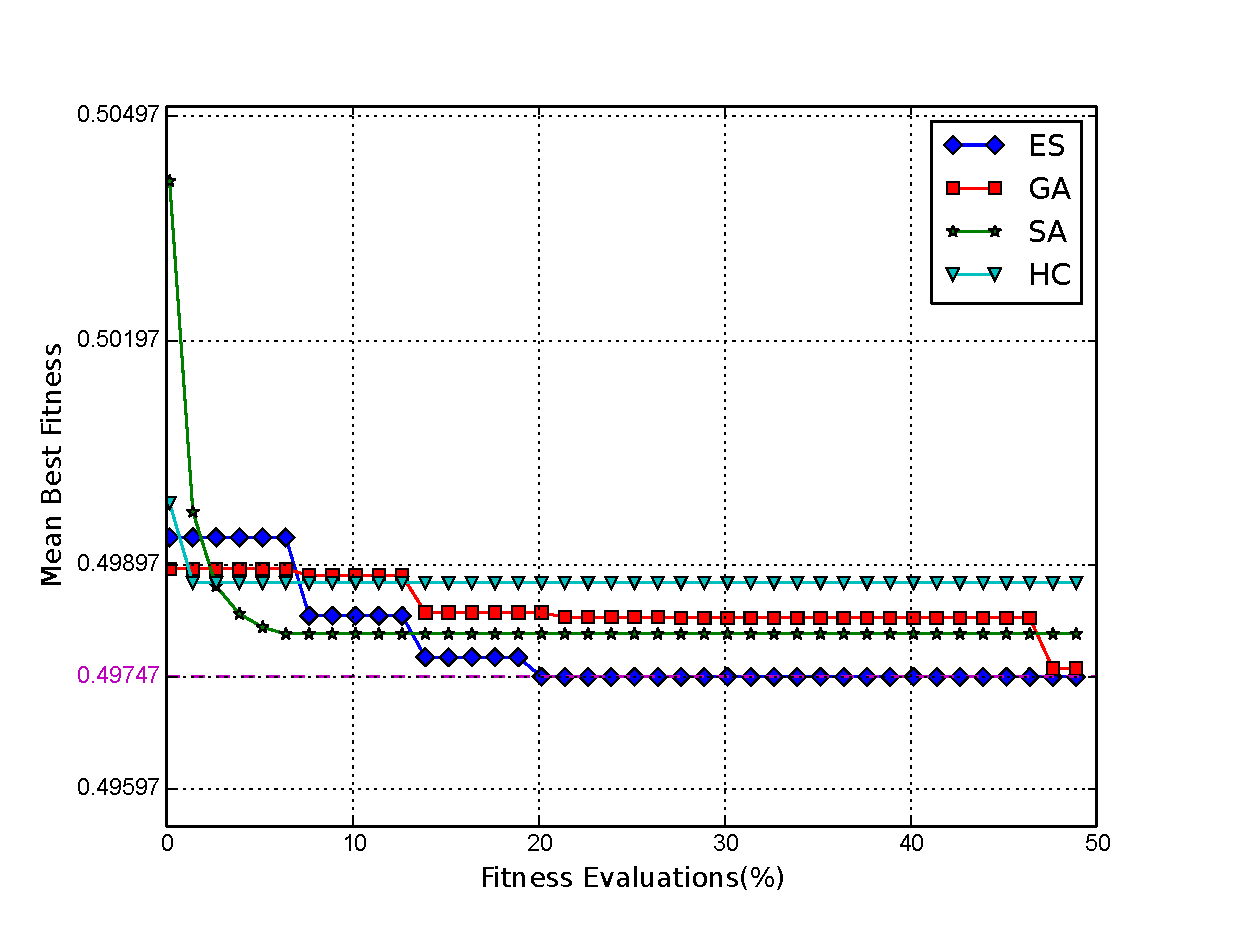
\includegraphics[trim=0 10 0 30,clip,height=5cm,width=8cm]{../paper/FIG/tc3_mf}%
            \end{figure}
        \end{column}
    \end{columns}
\end{frame}


\begin{frame}{Results - Test Case 4}
    \begin{columns}
        \begin{column}{\columnwidth}
            {\tiny Sample size = 1000}
            \adjustbox{max width=\columnwidth}{\tiny
                \begin{tabularx}{\columnwidth}{@{}l *4{>{\centering\arraybackslash}X}@{}} 
                    \toprule
                    Algorithm
                    & \multicolumn{2}{c}{\%Evaluations vs. Exhaustive}  
                    & \multicolumn{2}{c}{Best fitness}\\
                    \cmidrule(lr){2-3} \cmidrule(l){4-5}
                    & Mean & Std. Dev. &  Mean & Std. Dev. \\
                    \midrule
                    ES & 12.48 & 5.61 & 0.49926 & 0.00000 \\
                    SA & 2.76 & 0.83 & 0.49926 & 0.00000 \\
                    GA & 22.42 & 9.94 & 0.49934 & 0.00072 \\
                    HC & 0.44 & 0.26 & 0.49926 & 0.00000 \\
                    \bottomrule
                \end{tabularx}
            } \vspace*{-0.35cm}
            \begin{figure}
                \centering
                    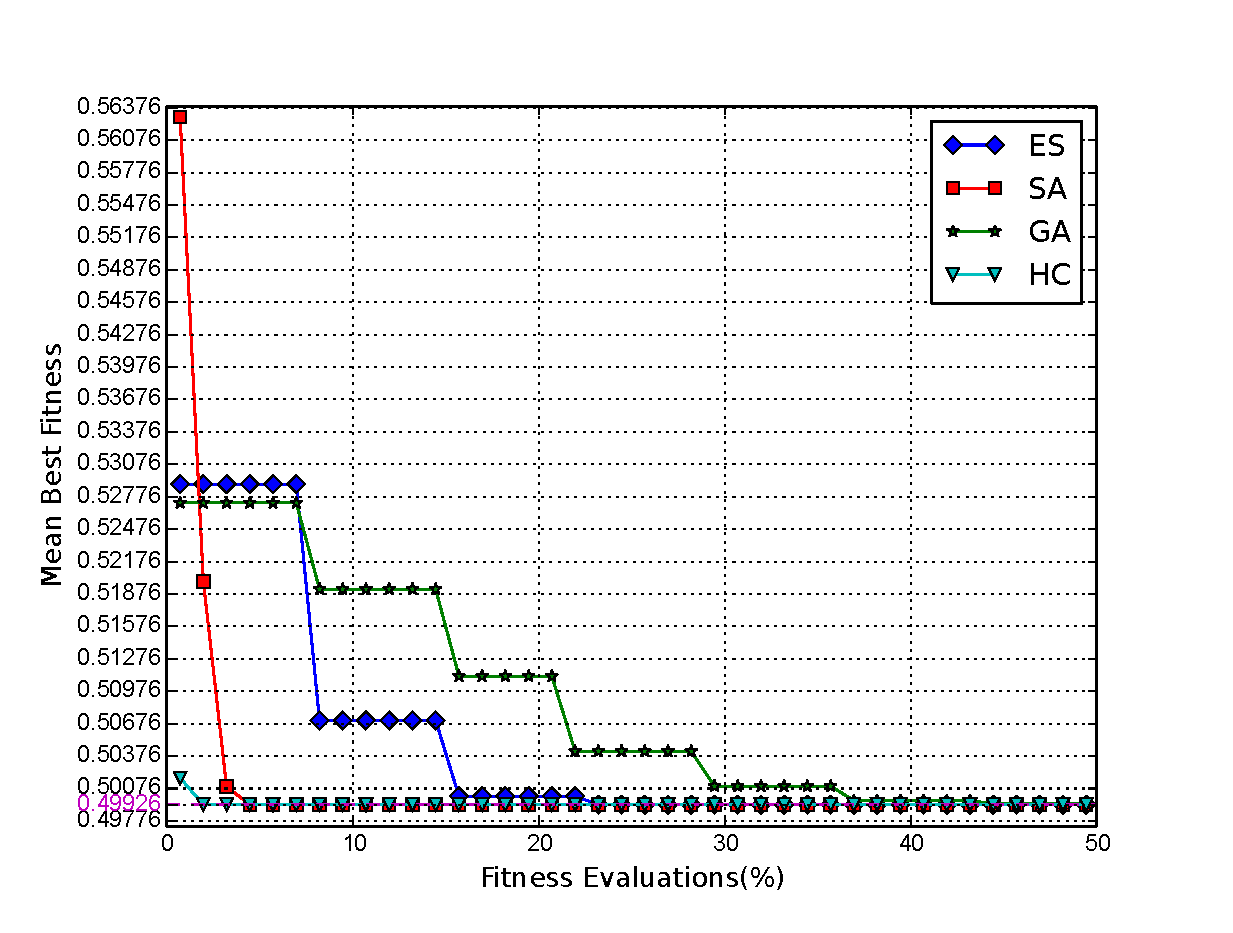
\includegraphics[trim=0 10 0 30,clip,height=5cm,width=8cm]{../paper/FIG/tc4_mf}%
            \end{figure}
        \end{column}
    \end{columns}
\end{frame}


\begin{frame}{Results - Success Rates}
    \textit{Success rate} reports percentage of runs in which the algorithm is able to find the optimum with $50\%$ evaluations as termination criteria
    \begin{figure}
        \vspace*{-0.35cm}
        \centering
        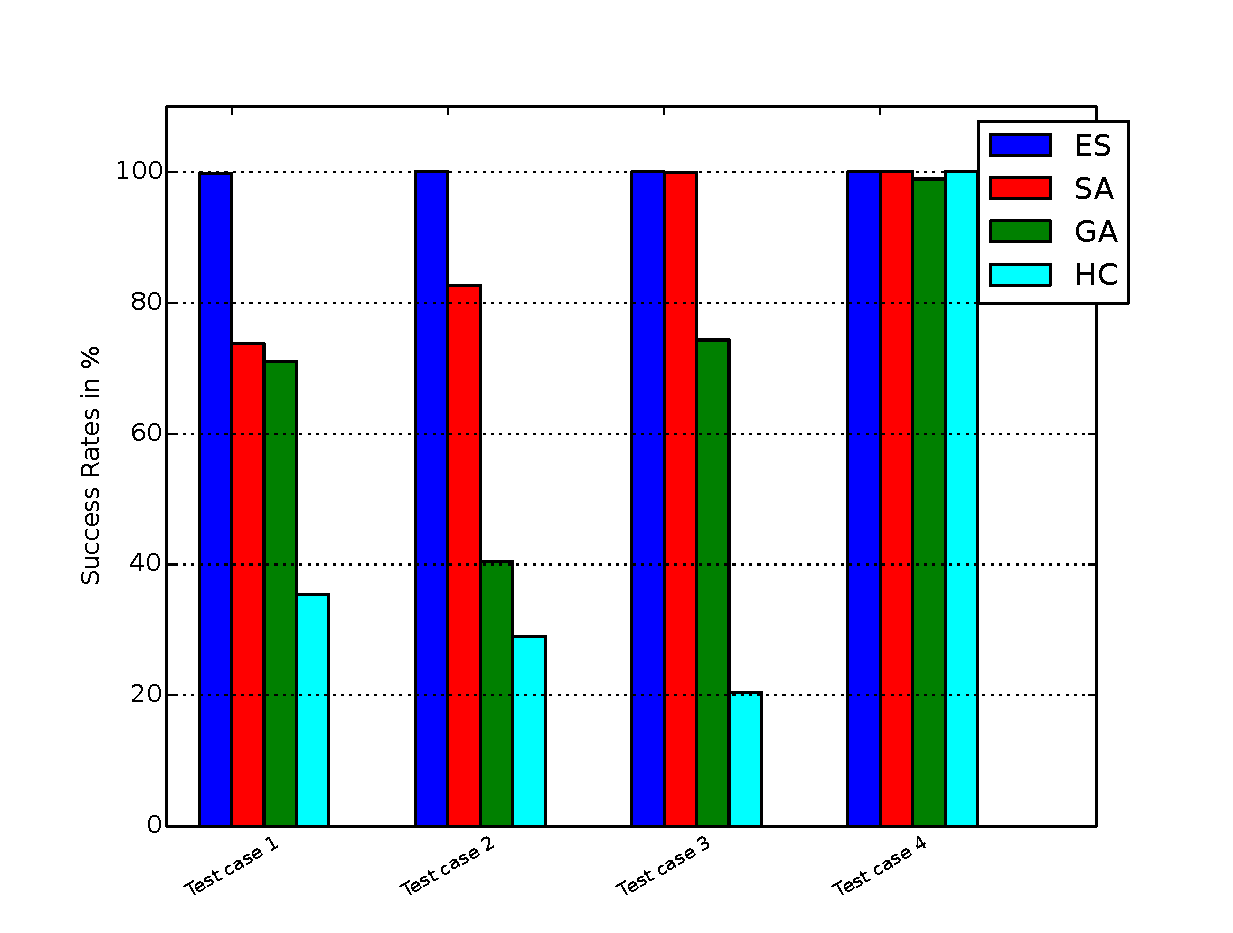
\includegraphics[scale=0.4]{../paper/FIG/tc_sp}
    \end{figure}
\end{frame}

\begin{frame}{Conclusions}
\begin{itemize} \itemsep1.5em
        \item First study to investigate optimizing multiple antenna placement on a single platform using multiple stochastic algorithms
        \item Formulated an automated procedure for the antenna placement problem which aims to improve the working of multiple antennas on a platform
    \end{itemize}
\end{frame}

\begin{frame}{Conclusions}
\begin{itemize} \itemsep1.5em
        \item Results show Simulated Annealing was less successful but faster to converge compared to Evolutionary Strategy
        \item Evolutionary Strategy was slower to converge but success rate $\approx100\%$ with a mean of at most $16\%$ evaluations of search space 
        \item Algorithms reduce search time to at most $1/4$ in comparison to an exhaustive algorithm
        \item Future work - Consider other techniques like \textit{Differential Evolution}, \textit{Particle Swarm Optimization} and \textit{ALPS}
    \end{itemize}
\end{frame}


\end{document}
